\documentclass[man,floatsintext,donotrepeattitle]{apa6}
%\documentclass[man,donotrepeattitle]{apa6}

% http://tex.stackexchange.com/questions/279/how-do-i-ensure-that-figures-appear-in-the-section-theyre-associated-with
\usepackage{placeins}

\usepackage[nodayofweek]{datetime}% http://ctan.org/pkg/datetime
\usepackage{xfrac}
\usepackage{textcomp}
\usepackage[american]{babel}
\usepackage[utf8]{inputenc}

% Single space after period (Mike prefers)
\frenchspacing

% http://tex.stackexchange.com/questions/36423/random-unwanted-space-between-paragraphs
\raggedbottom

% Changing horizontal space between subsubsection title and text, without loading titlesec package.
% Not loading titlesec because it clashes with apa6 package.
% Took base \@startsection command from apa6 .cls file, and tweaked horizontal spacing. 
% http://tex.stackexchange.com/questions/22576/redefining-sectioning-commands
% http://www.tex.ac.uk/cgi-bin/texfaq2html?label=atsigns
% http://tex.stackexchange.com/questions/60127/subsubsection-description-and-title-not-separated
\makeatletter
\renewcommand{\subsubsection}{%
  \@startsection
  {subsubsection}%
  {3}%
  {\parindent}%
  {0\baselineskip \@plus 0.2ex \@minus 0.2ex}%
  {-.4em}%
  {\normalfont\normalsize\bfseries\addperi}}
\renewcommand{\paragraph}{%
  \@startsection
  {paragraph}%
  {4}%
  {\parindent}%
  {0\baselineskip \@plus 0.2ex \@minus 0.2ex}%
  {-.4em}%
  {\normalfont\normalsize\bfseries\itshape\addperi}}
\makeatother

% ref: http://tex.stackexchange.com/questions/28516/how-to-change-the-title-of-toc
\addto\captionsamerican{% Replace ``english'' with the language you use
  \renewcommand{\contentsname}%
  {Table of Contents}%
}

%\usepackage[compact]{titlesec}
\usepackage{tabu}
\usepackage{amssymb,amsmath}
\usepackage{setspace}

% ref: http://tex.stackexchange.com/questions/48509/insert-list-of-figures-in-the-table-of-contents
\usepackage[nottoc,numbib]{tocbibind}

\usepackage[hyphens]{url}

% ref: http://tex.stackexchange.com/questions/73862/how-can-i-make-a-clickable-table-of-contents
\usepackage{hyperref}
\hypersetup{
  colorlinks,
  citecolor=black,
  filecolor=black,
  linkcolor=black,
  urlcolor=black
}
%\hypersetup{linktocpage}

%\usepackage{breakurl}
\usepackage{subfigure}
\usepackage{graphicx}

\usepackage[group-separator={,}]{siunitx}
\newcommand{\numNoZero}[1]{{\sisetup{add-integer-zero=false}\num{#1}}}

\newcommand{\myCI}[4]{{mean difference = \num{#1}, 95\% CI [\num{#2}, \num{#3}]}}

\RequirePackage[l2tabu, orthodox]{nag}
\graphicspath{{./figures/dissertation/}} % Specifies the directory where pictures are stored

\usepackage{csquotes}
\usepackage[style=apa,sortcites=true,sorting=nyt,backend=biber,doi=false,uniquename=false]{biblatex}
\DeclareLanguageMapping{american}{american-apa}

\addbibresource{bibliography.bib}

% Needed to ensure periods are placed at the end of every bibliography entry in the references section
\AtEveryBibitem{\clearfield{doi}}

% http://tex.stackexchange.com/questions/55780/disable-month-in-biblatex-bibliography
\AtEveryBibitem{\clearfield{month}}
\AtEveryCitekey{\clearfield{month}}

% Make sure only urls that are printed in references section are for webpages
\AtEveryBibitem{
  \ifentrytype{misc}{}{
    \clearfield{url}
  }
}

% ref: http://tex.stackexchange.com/questions/128592/remove-backslashes-from-url-fields-in-bib-entry
\DeclareSourcemap{
  \maps[datatype=bibtex]{
    \map{
      \step[fieldsource=url,
	match=\regexp{\\},
      replace=\regexp{}]
    }
  }
}

% Do not let biblatex change any of the casing in the bibliography file
\DeclareRobustCommand{\MakeSentenceCase*}[1]{{#1}}

% Customer citation for a parencite style but with a few leading words in the parentheses
% Stolen from parencite but with the out parentheses stripped off
% For example: (e.g., Anderson, 1972), (see Salton, 2014)
\DeclareCiteCommand{\noparencite}
  {\usebibmacro{prenote}}
  {\usebibmacro{citeindex}%
   \usebibmacro{cite}}
  {\multicitedelim}
  {\usebibmacro{postnote}}


% If the toc is too detailed, try limiting the depth of printed sections in the TOC:
\setcounter{tocdepth}{2}

\title{Comparing vector-based and Bayesian memory models using large-scale datasets:\protect\\User-generated hashtag and tag prediction on Twitter and StackOverflow}
\shorttitle{Comparing memory models of tag retrieval}
%\shorttitle{}

\author{Clayton Stanley and Michael D. Byrne}
\affiliation{Rice University}

\leftheader{Beitzel}

\keywords{ACT-R declarative memory theory, vector-based models, LSA, machine learning}

\begin{document}

\abstract{
  The growth of social media and user-created content on online sites provides unique opportunities to study models of human declarative memory.
  By framing the task of choosing a hashtag for a tweet and tagging a post on StackOverflow as a declarative memory retrieval problem,
  two cognitively-plausible declarative memory models were applied to millions of posts and tweets and evaluated on how accurately they predict a user's chosen tags.
  An ACT-R based Bayesian model and a random permutation vector-based model were tested on the large datasets. 
  The results show that past user behavior of tag use is a strong predictor of future behavior.
  Furthermore, past behavior was successfully incorporated into the random permutation model that previously used only context.
  Also, ACT-R's attentional weight term was linked to an entropy-weighting natural language processing method used to attenuate high-frequency words (e.g., articles and prepositions).
  Word order was not found to be a strong predictor of tag use, and the random permutation model performed comparably to the Bayesian model without including word order.
  This shows that the strength of the random permutation model is not in the ability to represent word order, but rather in the way in which context information is successfully compressed.
  The results of the large-scale exploration show how the architecture of the two memory models can be modified to significantly improve accuracy,
  and may suggest task-independent general modifications that can help improve model fit to human data in a much wider range of domains.
}

%\note{\today}

\maketitle

%\newpage

\section{Introduction}

With the massive growth of human-created content on social media sites (e.g., Twitter, StackOverflow, Wikipedia) and public access to many of those databases,
it is now possible to evaluate psychological theories of declarative memory on large-scale real-world tasks where the theory can be tested on hundreds of millions to billions of data points.
Without using large datasets it is difficult to verify and explore modifications to the declarative memory architecture because the datasets are not large enough or rich enough to rigorously test modifications to the theory.

A few researchers have started to use large-scale databases to evaluate how well declarative memory models scale,
for both ACT-R Bayesian models \parencites{Fu2007,Pirolli2003,Stanley2013,Douglass2010} and vector-based memory models \parencites{Jones2007,Rutledge2008,Recchia2010,Sahlgren2008}.

This study expands on previous work that has tested retrieval models on large-scale datasets.
It focuses specifically on how two state-of-the-art declarative memory retrieval models (ACT-R Bayesian and random permutation vector-based) can be improved by testing these models on two real-world tagging tasks.
One primary objective is to compare the random permutation vector-based model to ACT-R's Bayesian declarative memory theory when large datasets are used for each model. 
Another objective is to improve each model, and measure how incorporating the strengths of each model into the other (i.e., modifying model components) influences accuracy.
For example, modifying a vector-based model to retrieve results that are based not only on context, but also on the prior odds that a particular item in memory will be needed again.
Large-scale datasets were used throughout the model development and evaluation process.
This provides an ideal testing environment for constraints and assumptions for each theory to be rapidly tested and new model components to be hypothesized and quickly evaluated.

As a general methodology for this research, we used a cognitively-constrained exploratory model development process.
Since we worked with large-scale datasets, we had enough data to explore many different modifications simultaneously without the risk of overfitting.
However, we were not interested in bringing to bear the entire collection of machine learning algorithms to this prediction task in order to completely optimize a model.
Rather, we were interested in evaluating how well two cognitive models could explain the results, and then making selective modifications to them to see how performance changes.
The modifications that we explored were selected such that they influenced model accuracy, could be easily added to (or removed from) the cognitive models without massive modifications, and could be considered cognitively plausible.

\subsection{Research Questions}

The core question motivating this research is:
What kinds of cognitively-plausible models can best predict the tags that a user on a social media site selects?
This question can be tested by generating a prediction for the most likely selected tag whenever a user is about to generate a tag, and then comparing the user's chosen tag to the model's prediction.
The process of suggesting a relevant tag to a user can be thought of as a memory retrieval request for a tag, given prior tag use and current context.

Co-occurrence-based modeling has been shown as a potentially useful approach when predicting Twitter hashtag selection \parencite{Efron2010} and StackOverflow tag selection \parencites{Stanley2013}.
Several memory retrieval models are based on this broad methodology, where a count is maintained of the times each contextual element (such as a word in a post) co-occur with a tag.
At least two of the current memory retrieval models are based on a co-occurrence methodology:
ACT-R's declarative memory (DM) retrieval theory and random permutation vector-based memory systems.

\subsubsection{StackOverflow and Twitter}

These two memory models were compared across two domains where users generate tags for posts: Twitter and StackOverflow.
Twitter is a microblogging service where users create 140 character ``tweets'' and broadcast those messages out to the users who follow their posts.
A user is free to annotate important concepts or words in the tweet by preceding words with ``\#,'' thereby making the word into a hashtag.
After the tweet is created the hashtags become hyperlinks, and if clicked on will take a user to a summary feed of all of the tweets across Twitter that have used that hashtag.
Some recent and often used hashtags for Twitter are \emph{\#photography}, \emph{\#startup}, \emph{\#4change}, \emph{\#android}, and \emph{\#solar}.

The two memory retrieval models were also tested on tag selection for StackOverflow posts.
StackOverflow is a question and answer site for computer programming where users ask programming-related questions and fellow members of the community provide answers.
A user with a programming-related question creates a post with their question and tags the post with a few specific programming-related tags. 
The tags chosen by a user on the StackOverflow site represent the primary topic of the question, such as a specific programming language, tool, software package, or framework.
Some example tags for StackOverflow are \emph{PHP}, \emph{Arrays}, \emph{MVC}, \emph{C\#}, and \emph{Common Lisp}.

The StackOverflow and Twitter datasets were chosen because the human-created content between them is quite different, and were interested in retrieval models that generalize across tasks.
However, they are also similar on several accounts:
Both domains have amassed large amounts of user-created content, users generate tags for posts when creating content on the site (hashtags for Twitter and tags for StackOverflow),
and the user data from the datasets are publicly available for analysis.

\subsection{Roadmap}

This rest of this document is separated into 5 sections.
``Theoretical Background'' describes the vector-based and Bayesian declarative memory models that were evaluated in this research,
shows how these models are related to the other common declarative memory models,
and identifies examples of similar tagging models that have already been applied to various tag recommendation systems.
``General Methodology'' presents the overall method for testing the models on the StackOverflow and Twitter datasets.
``Past User Behavior'' shows the results for the first test of the models, where the model term for past user behavior is examined in isolation, and tags are predicted based purely on a user's past tagging history.
``Combining Predictors'' adds the context component to the models, and shows how model accuracy is influenced by changing various architectural components of each model.
The final section provides a general discussion of the overall findings.

\section{Theoretical Background}

\subsection{ACT-R Declarative Memory Theory}

ACT-R \parencite{Anderson2007} is a cognitive architecture that formalizes how each cognitive process of the mind (e.g., memory, learning, visual and motor) interacts to produce behavior.
The declarative memory system is a component of the architecture that models the timing, learning, and forgetting processes that make up declarative memory storage and retrieval.
At the core of the system is the concept of a ``chunk'': the representation of a piece of knowledge (e.g., a word).
The equations that make up this system were derived from a rational analysis of declarative memory retrieval \parencite{Anderson1989}.
That is, given the task of retrieving a chunk of information from declarative memory,
the current context (i.e., external and internal environment state), and past experience (i.e., prior memories and exposure), 
what is the optimal behavior (i.e., the optimal chunk to retrieve from memory)?
Using Bayesian reasoning, each chunk of information in declarative memory can be assigned a prior likelihood of needing retrieval again, given the prior history of exposure to the chunk.
These chunk prior probabilities are then adjusted for the current context, so that the posterior probabilities represent the likelihood that a chunk is needed, given prior odds and adjusted by current environment state.

\subsubsection{ACT-R DM Model}

A formal description of the ACT-R Declarative Memory model is included in Table \ref{tabACTRModel}.

\begin{table}[!ht]
  \caption{ACT-R declarative memory model}
  \label{tabACTRModel}
  {\tabulinesep=1.2mm
    \begin{tabu}{ll}
      \hline
      Common Name &  Equation \\
      \hline
      Activation &	 	$A_{i} = B_{i} + \sum_{j \in c}^{} W_{j} S_{ji}$ \\
      Attentional Weight &	$W_{j} = \frac{W}{n}$ \\
      Base Level & 		$B_{i} = log \sum_{j=1}^{n} {t_{j}}^{-d}$ \\
      Strength of Association &	$S_{ji} = log \frac{p(i|j)}{p(i|\overline{j})} \approx log \frac{p(i|j)}{p(i)} = log \frac{NN_{ji}}{N_{Row}(j)N_{Col}(i)}$ \\
      Recall Probability &	$P_{i} = \left( 1 + e^{\frac{\tau - A_{i}}{s}} \right )^{-1}$ \\
      \hline
    \end{tabu}
  }
\end{table}

The total activation ($A_{i}$) for a chunk in declarative memory is a function of two components: base-level activation ($B_{i}$) and strength of association ($S_{ji}$).
The recall probability ($P_{i})$ that a chunk will be retrieved from memory increases with total activation ($A_{i}$).
Each term in Table \ref{tabACTRModel} will be discussed in greater detail to follow.

\subsubsection{Base-Level Activation}

Base-level activation reflects the log prior odds of needing an observed chunk again.
The default way to calculate these log prior odds is to use the standard base-level equation in Table \ref{tabACTRModel}.
This equation formalizes how log prior odds are a function of both frequency and recency of prior exposure to a particular chunk.
Chunks used more frequently (either through exposure or from a retrieval) are more likely to be needed for retrieval again.
However, as time progresses and a particular chunk is no longer used, the activation for that chunk decays.
In this way the standard base-level equation formalizes the time dynamics of the retrieval system, where a chunk's base-level activation evolves over time, depending on its frequency and recency of use.

\subsubsection{Strength of Association}

Strength of association ($S_{ji}$) reflects the amount of log-odds adjustment to the activation of a chunk, given the current context (i.e., external environment and internal state).
Context for the StackOverflow domain for example is represented as each word in the title and body of a post.
Context for the Twitter domain are the words in a tweet.
Association strength between a chunk in memory and a single contextual element can be computed directly by calculating its context-adjusted odds ratio:
the likelihood a chunk occurred with the current context ($p(i|j)$) over the likelihood that the chunk occurred in any of the other contexts ($p(i|\overline{j})$).
For large datasets, the likelihood that a chunk occurs in any particular context reaches near-zero values ($p(j) \Rightarrow 0$).
So it can be assumed that the likelihood that a chunk occurs in any context but one ($p(i|\overline{j})$) is equivalent to the likelihood that a chunk occurs in any context ($p(i)$).
This assumption was described when deriving the $S_{ji}$ equation \parencite{Anderson1989}, and used in recent research working with large-scale datasets \parencites{Stanley2013,Farahat2004,Douglass2010}.

\subsubsection{Connection to Pointwise Mutual Information}

Pointwise Mutual Information (PMI) is another co-occurrence index that measures strength of association between two terms \parencite{Farahat2004}.
It is based on the co-occurrence count between pair-wise observations of terms, similar to ACT-R's strength of association.
The index has been used to accurately and efficiently measure strength of association information for large-scale datasets \parencite{Budiu2007,Farahat2004}.
The PMI index is presented as Equation \eqref{eqPMI}.

\begin{equation}
  \label{eqPMI}
  \mathit{PMI}(y,x) = log \frac{p(y|x)}{p(y)}
\end{equation}

Further, this PMI equation is identical to ACT-R's strength of association ($S_{ji}$) equation for large datasets.
Once the number of occurrences is large enough such that the probability of observing any particular contextual element ($p(x)$) is near zero, then ACT-R's strength of association index simplifies to the PMI equation.

\subsubsection{Attentional Weight}

The attentional weight term allows for some contextual components to be weighted more than others when the total $S_{ji}$ activation is computed.
This reflects the fact that the declarative memory system has limited attentional resources ($W$) that must be spread across all of the items in context.
Most ACT-R models simply weight each contextual element equally (e.g., all words in a StackOverflow post have equal weight), so each word's attentional weight is simply normalized by the number of items in context.

\subsection{Vector-Based Memory Systems}

``Holographic'' memory systems \parencite{Plate1995} or vector-based memory systems represent a concept (i.e., a chunk) as a vector.
The representation of the concept is distributed across all elements of the vector.
This is somewhat similar to taking a column (i.e., a tag) on a word co-occurrence matrix and viewing the distribution of co-occurrence counts across the rows in the column as the representation of that concept.
However, vector-based memory systems represent information in a much more compact way than a full word co-occurrence matrix.

For vector-based systems, each word is represented by an environment vector $e_{i}$ that is nearly orthogonal to all other words' environment vectors.
The number of dimensions for these vectors is much less than the number of rows in a full word co-occurrence matrix (typically around 2,000 - 4,000), which is how vector-based systems represent information in a much more compact space.
Paired with each environment vector ($e_{i}$) is a memory vector ($m_{i}$) that contains the summed representation of all other environment vectors that have co-occurred with that $e_{i}$ environment vector.
These memory vectors can contain environment vectors from position-independent word co-occurrence information ($c_{i}$) and word order information ($o_{i}$), which can be combined into a single representation ($m_{i}$).
Over time, memory vectors accumulate a distributed representation of the most common environment vectors that co-occurred with them.

\subsubsection{Retrieval Process}

Retrieving the most likely chunk given context can be done in two ways: decoding and resonance \parencite{Jones2007}.
Decoding takes the memory vector for context and decodes it back into an environment vector.
The cosine between that decoded environment vector and all other environment vectors is computed and ranked, and the chunk with the environment vector with the highest cosine is retrieved.

Resonance is the opposite retrieval process, where a memory vector is created from the context, and then that context memory vector is compared to all memory vectors.
For example, assume that a user has written the word ``zend'' in a post, and she wants to assign a tag for the post.
``zend'' has co-occurred with the tag \emph{PHP} many times previously, so the unordered memory vector for ``PHP'' ($c_{\mathit{PHP}}$) contains the unordered environment vector for \emph{zend} ($e_{zend}$).
To determine the most correlated memory vector with context, a memory vector is created from the current context ($e_{zend}$).
The cosine between that context memory vector and the memory vector for \emph{PHP} will be high, since the \emph{PHP} memory vector ($c_{\mathit{PHP}}$) often contains the context environment vector ($e_{zend}$).
Since the cosine is high, the tag \emph{PHP} will most likely be returned as the vector that resonates highest with the current context.

The resonance and decoding processes are inversions of each other.
Usually both resonance and decoding will return similar rank orderings of most likely chunks given context.

\subsubsection{Word Order for Vector-Based Systems}

One of the strengths of vector-based systems is that word order can naturally be represented alongside word co-occurrence in these distributed representations.
With vector-based systems, order information is included by creating an environment vector ($e_{bind(i,\Phi)}$) that is a function of environment vectors for both the word ($e_{i}$) and location ($\Phi$).
This function has the useful property that the resulting environment vector and the location vector can be inverted to return the original word's environment vector.
Circular convolution and inverse circular convolution (i.e., circular correlation) are used by \textcite{Plate1995} and \textcite{Jones2007}'s BEAGLE model to implement these operations.
This allows for retrieval requests such as ``playing \#$\Phi$,'' ``just read \#$\Phi$,'' and ``vector-based $\Phi$ systems.''

\subsubsection{Random Permutation Model}

In order to represent word order information, a function must be used that converts an environment vector for a set of words and positions (e.g., ``stack $\Phi$'') into a new uncorrelated environment vector.
\textcite{Sahlgren2008} used a simple random permutation method for this operation.

A formal description of the random permutation model in \textcite{Sahlgren2008} is included in Table \ref{tabRandPermModel}.
With random permutations, each word environment vector ($e_{i}$) is a large sparse vector of zeros with a few one and negative one values in random locations. 
In order to create a new environment vector for a word that preceded another word in a sentence, that word's environment vector is shifted to the left one position.
This produces a new environment vector ($e_{i^{-1}}$) for the combination of the word and the position that is uncorrelated with the original word's environment vector and all other environment vectors.

\begin{table}[!ht]
  \caption{Random permutation model}
  \label{tabRandPermModel}
  {\tabulinesep=1.2mm
    \begin{tabu}{ll}
      \hline
      Common Name &  Equation \\
      \hline
      Activation &		$A_{i} = r(m_{C},m_{i})$ \\
      Memory Vector &		$m_{i} = \sum_{i \in all past} c_{i} + \sum_{i \in all past} \sum_{l \in locations} o_{i,l}$ \\
      Unordered Context &	$c_{i} = e_{i}$ \\
      Ordered Context &		$o_{i,l} = e_{i^{-l}}$ \\
      Context Memory Vector &	$m_{C} = \sum_{i \in C} c_{i} + \sum_{i \in C} \sum_{l \in locations} o_{i,l}$ \\
      Environment Vector & 	$e_{i} = rand$ \\
      \hline
    \end{tabu}
  }
\end{table}

\subsubsection{Connection to LSA}

Latent Semantic Analysis \parencite{Landauer1997} (LSA) is an alternative representation of declarative memory.
Both vector-based models and LSA calculate word similarity on a reduced matrix.
For LSA, the original word by document matrix is compressed to a factor by document matrix and the number of factors is much less than the number of words.
LSA uses Singular Value Decomposition (SVD) to find words that have highly correlated document occurrence distributions (i.e., latent concepts), and then pools those co-occurrence counts into a single dimension.

For vector-based models, each tag (document) is represented by a compressed vector with a length much less than the number of words.
A vector-based approach like random permutations essentially randomizes the mapping of the words on the reduced set of dimensions, and does not take into account word similarity when generating the mapping.
Nonetheless, vector-based models have been shown to perform similar to if not better than LSA \parencites{Sahlgren2008,Jones2007}.

\subsection{Comparison of Vector-Based Models and ACT-R}

Vector-based models can be thought of as a compressed representation of the full co-occurrence matrix used for the ACT-R declarative memory system.
Each model computes an activation for each word to retrieve, given context and (for ACT-R's Bayesian model) prior knowledge.
Since both models produce activations for each chunk, one can be swapped out for another and used as the declarative memory component of the ACT-R infrastructure.
For example, \textcite{Rutledge2007} used a variant of the BEAGLE vector-based model as the DM component of ACT-R.
\citeauthor{Rutledge2008} showed that an ACT-R theory with a vector-based memory system can successfully model the fan effect \parencite{Anderson1974}.

\subsubsection{Base-Level Activation}

Vector-based models and ACT-R's Bayesian DM model are not identical however, and these differences need to be addressed in order to better evaluate the relative benefits of the two models. 
In particular, the frequency and recency of retrievals for each chunk are not currently used for vector-based models when calculating activation.

The frequency and recency of how content has been used in the past can be a strong predictor of the future importance of that information. 
The recent content in tweets on a news site like Twitter should be more relevant, for example.
\textcite{Efron2011} tested this claim by evaluating a set of query likelihood models on returning relevant Twitter tweets from search queries.
They showed that a model incorporating recency information of the tweet produced more relevant results than models that did not pay attention to this information.

ACT-R's Bayesian model has a strong theory with respect to recency and frequency information.
It uses this information to calculate a chunk's prior activation (i.e., prior likelihood of being needed again, independent of current context).
Vector-based models compute activation based entirely on context, so chunks that resonate with context will be retrieved, irrespective to the frequency and recency of use of that chunk.
ACT-R's prior activation can also be computed for each user, so that hashtags that have been used frequently and recently for a particular user are rated with higher activation.
Vector-based models have focused on computing the associative strength of a chunk and specific contextual elements.
It is unexplored how accuracy changes for these models once the information about a user's prior behavior (e.g., ACT-R's base-level activation component) is added.

\subsubsection{Word Order}

One strength of a vector-based approach over ACT-R's Bayesian DM model is that word order can be naturally represented alongside unordered co-occurrence information.
With the ACT-R model, for example, it is unclear how to represent that a particular word appeared just before a hashtag. 
To represent word order in a Bayesian model, an additional dimension could be added to the co-occurrence matrix that represents word position.
However, adding word-order information to ACT-R's default Bayesian declarative memory model is not common.
Instead, when word order information is used to model reading for example, production rules are defined so that words are read from left to right (e.g., \noparencite{Lewis2006}).

\subsubsection{Activation Calculation}

Vector-based retrieval models calculate chunk activation by correlating a representation of the current context with each memory item.
Bayesian retrieval models like ACT-R calculate activation by computing each chunk's posterior odd adjustment likelihood, given the context.
These two computations are certainly not equivalent, even though they are most likely correlated with one another.

Using a correlation can be problematic due to range effects in observed co-occurrences.
If there are particular words for a tag that co-occur much more often than all of the other words with that tag, that single large value diminishes the power of all other words to contribute to the correlation calculation.
This does not happen with Bayesian retrieval models because each pair of word and tag values is normalized by the total number of words that appeared with that tag and total number of tags that appeared with that word
(see the strength of association equation in Table \ref{tabACTRModel}).
The high-frequency words are often removed from the co-occurrence matrix for vector-based models to reduce this effect.

\subsection{Hashtag Prediction}

Models that attempt to predict a user's chosen hashtag have recently been created and tested for a few social media sites,
though most of these models are not based on theories of human declarative memory.
Google has even deployed a hashtag recommendation model to help users properly tag posts on their Google+ social media site \parencite{GoogleKeynote2013}.
A tag-suggestion tool has also been deployed for the \url{tex.stackexchange.org} and \url{superuser.com} StackExchange sites.
Models for Twitter and StackOverflow have been proposed and tested, but none have yet been deployed.
Recommendation models for StackOverflow and Twitter will be described in more detail to follow.

\subsubsection{StackOverflow}

\textcite{Stanley2013} used a declarative memory model to predict a user's chosen tags for a post on the StackOverflow site.
They modified the standard ACT-R model in order to more accurately predict tag use on StackOverflow.
A formal description of the modified ACT-R Bayesian model is included in Table \ref{tabModACTRModel}.

\begin{table}[!ht]
  \caption{\citeauthor{Stanley2013}'s StackOverflow tag prediction model}
  \label{tabModACTRModel}
  {\tabulinesep=1.2mm
    \begin{tabu}{ll}
      \hline
      Common Name &  Equation \\
      \hline
      Activation & 		$A_{i} = B_{i} + \sum_{j\in T}^{ } W_{j} S_{ji} + \sum_{j\in B}^{ } W_{j} S_{ji} - O$ \\
      Base Level & 		$B_{i} = log \frac{p_{i}}{1-p_{i}}$ \\
      Strength Assoc. &		$S_{ji} = log \frac{p(i|j)}{p(i))} = log \frac{NN_{ji}}{N_{Row}(j)N_{Col}(i)}$ \\
      Attentional Weight & 	$W_{j} = W \frac{E_{j}} {\sum_{}^{} {E_{j}}} $ \\
      Scaled Entropy & 		$E_{j} = 1-\frac{H_{j}}{H_{max}}$ \\
      Entropy & 		$H_{j} = -\sum_{i=1}^{N}p(i|j)log\left (  p(i|j) \right )$ \\
      \hline
    \end{tabu}
  }
\end{table}

The activation of each tag ($A_{i}$) is a function of four components:
That tag's base-level activation ($B_{i}$), contextual activation for the words in the title, activation for words in the body, and an offset term ($O$).
This model has been modified from the standard ACT-R model in four ways:
Two separate contextual components were used (words in title and body of post), an offset term was added, an entropy measure was used to compute the attentional weight ($W_{j}$),
and the base-level activation of a tag was based on global past tag use and not customized to a user's past tagging history.

The offset term was added to normalize the mean activation across retrievals.
This allowed the use of a logistic regression statistical technique to calibrate the weights for each of the terms.
The scaled entropy measure $E_{j}$ was chosen for the attentional weight ($W_{j}$) term because it has a strong theoretical foundation \parencite{Dumais1991} and is parameter-free.

\subsubsection{Twitter}

Several hashtag recommendation models for Twitter have been developed recently.
One of the first models used a Bayesian co-occurrence statistical technique to predict the most likely hashtag associated with a tweet as a function of prior hashtag use and context \parencite{Mazzia2009}.
This is quite similar to an ACT-R declarative retrieval model.
The main potential difference is that---like \textcite{Stanley2013}---the global prior likelihood of a hashtag is computed without taking into account the specific user's past history.

Several other models have taken a tweet-centered approach to hashtag prediction, where suggested hashtags are collected from hashtags used in similar tweets.
\textcites{Li2011, Zangerle2011, Kywe2012} all store a content vector for each tweet, and then compute a word co-occurrence-based similarity score between a composed tweet and the rest of the tweets in the database.

There has been a mix of co-occurrence models created to predict hashtag use on Twitter, and the results are encouraging.
However, there has been little research on how a specific user's past hashtag use should influence the model's prediction when that user is composing a tweet.
\textcite{Kywe2012} did take a user-centered view with their model, but the hashtags predicted by the user and content were analyzed separately and then the top from each group were combined for prediction.
The ACT-R declarative memory retrieval theory shows how past experience and current context combine to produce the most likely retrieval.
Each component is summed together to generate a total activation, and then the likelihood of chunks are ranked by that summed activation.
This technique is compensatory and allows for a more natural combination of the two components, where weights can be assigned to each component depending on how strongly each term predicts performance.

\section{General Methodology}

Different subsets of the StackOverflow and Twitter datasets were used to evaluate past user behavior in isolation and to test the context component of each memory model.
These datasets will be named and described in general terms.
Also, the general methods used to tokenize and stem the words in all of the datasets will be described.
All software code created for this research is publicly available on GitHub \parencite{StanleyRepo2014}.

\subsection{Models}

Two models were evaluated for hashtag prediction on both the Twitter and StackOverflow datasets:
the random permutation vector-based model \parencite{Sahlgren2008} in Table \ref{tabRandPermModel} and 
the modified ACT-R Bayesian model \parencite{Stanley2013} in Table \ref{tabModACTRModel}.

\subsection{Datasets}

The most recent quarterly published StackOverflow dataset \parencite{DataDump2014} was used to test the models on user chosen tags for posts.
This dataset contains around \num{5.7} million posts and \num{34377} unique tags.

Unlike StackOverflow, the entire Twitter dataset is not released to the public.
Due to this and the scale of Twitter, only subsets of the Twitter dataset were examined.
The relevant subsets are described below.

\subsubsection{Popular Users Dataset}

A popular-users dataset was collected for both StackOverflow and Twitter.
This dataset consists of all of the tweets and posts from various samples of the top users for each site.
This dataset was collected by fetching all past tagging history for each of the top users.
It was used to explore the growth and decay characteristics of a hashtag for individual users.
The temporal dynamics of ACT-R's decay rate model for a chunk were evaluated against these data.
Multiple samples were taken across a broad range of user types for each dataset to ensure that the model results were not dependent on specific attributes in a single sample.

For StackOverflow, top users were identified by their reputation score on the site (based on their upvoted questions and answers) and the total number of questions asked on the site.
To create the StackOverflow popular-users dataset, a total of 12 slices of users were taken at different levels of reputation and total number of questions asked.
500 users were sampled that had a reputation higher than \num{500}, \num{1000}, \num{5000}, \num{10000}, \num{50000}, and \num{100000}.
100 users were sampled that had asked a total number of questions higher than \num{50}, \num{100}, \num{200}, \num{300}, \num{400}, and \num{500}.

For Twitter, top users were those that had the largest number of followers and had authored the largest number of tweets.
To create the Twitter popular-users dataset, 12 slices were also taken, this time at different levels of number of followers and total number of tweets.
100 users were sampled that had a total number of followers higher than \num{1000}, \num{5000}, \num{10000}, \num{100000}, \num{1000000}, and \num{10000000},
and a total number of tweets higher than \num{100}, \num{500}, \num{1000}, \num{5000}, \num{10000}, and \num{50000}.

\subsubsection{Popular Hashtags Dataset}

An additional popular-hashtags dataset was collected for Twitter.
This dataset was used to test the context component of the models for Twitter.
The dataset contains approximately three million tweets where at least one of the 400 most popular hashtags are used.
A quota of three million tweets was selected because previously research testing Bayesian co-occurrence models on large-scale datasets has used on the order of one million documents
\parencites{Stanley2013,Douglass2010,Budiu2007}.
Tweets were collected in real time until the tweet quota was reached.

Four popular-hashtags datasets were collected at four different time periods, spanning one month.
Multiple datasets were collected to ensure that the results were not dependent on a particular sample of hashtags and would generalize across different popular-hashtag datasets and different time periods.
Each dataset required around four days to collect enough tweets to reach the quota, and one collection was done each week.

\subsubsection{Randomly Sampled Dataset}

Since the entire dataset is available for StackOverflow, randomly-sampled posts were used to test the context models rather than creating a popular-tags dataset (analogous to Twitter).
If all Twitter data were available, then the models would have been tested on a randomly-sampled dataset for Twitter as well.
However, since this is not the case for Twitter, the popular-hashtags dataset was used instead of a randomly-sampled dataset for that site,
while models for StackOverflow were tested on the more challenging dataset where posts were randomly sampled across all posts created on the site.

\subsection{Acquiring Datasets}

\subsubsection{StackOverflow}

The entire StackOverflow dataset is packaged and released quarterly to the public,
so the most recent packaged dataset was downloaded and the tables were imported into a relational database.

\subsubsection{Twitter}

Twitter provides two types of APIs for acquiring data: one based on streaming and a direct query-based interface.
The query-based interface was used to collect all tweets for specific popular users.
At most \num{3000} of the most recent tweets were collected for each user, since Twitter only allows access to this number of tweets for each user.

The streaming interface was used to collect a sample of all of the tweets that included one of the top 400 hashtags at that time.
Twitter's streaming API only allows at most 400 hashtags to be monitored at a time.
Otherwise a larger number of hashtags would have been collected.
Twitter limits the streaming interface to randomly sample about 1\% of all of the real-time data that is generated on Twitter.
This sampling rate was adequate to collect around three million tweets within a few days.

\subsection{Tokenization}

A custom tokenization algorithm created by \textcite{Owoputi2013} was used to parse the words in the text.
This algorithm was specifically created for tokenizing Twitter content.
However, during testing it was also found to be robust and well-suited for StackOverflow content.
The initial model results with the new tokenizer were qualitatively similar to the model results found in \textcite{Stanley2013} where the Python Natural Language Processing (NLP) toolkit \parencite{Bird2009} was used.
The same tokenization algorithm from \textcite{Owoputi2013} was used for both StackOverflow and Twitter to make comparisons across datasets more equitable.

\subsection{Stemming}

\textcite{Owoputi2013}'s algorithm handles basic word stemming (e.g., removing ``ed'' and ``ing'' endings).
With the StackOverflow dataset however, it is also possible to convert synonym tags to canonical base tags, since the community maintains a tag-synonym database.
This can be thought of as semantic stemming, where two words with identical meaning are converted to the same canonical word.
So tags used for the post were converted to their root tag when possible.
This does make the decision process easier for the StackOverflow dataset.
However, we chose to include this to help ensure that model predictions would stabilize.
This provided the best opportunity to reliably observe differences in accuracy when altering the models. 

\subsection{Testing for Reliable Differences}

In similar spirit to \textcites{masson2003using, tryon2001evaluating, cumming2005inference}, confidence intervals were used throughout for statistical inference instead of explicit $p$-values.
This was done because it is a more straightforward way to visualize all of the mean differences in accuracy (i.e., bar and line plots with a visual indication of the error) for each of the models, which eases interpretation.
It is also a conservative estimate of reliability, as using confidence intervals on the means essentially ignores the fact that this is a within-subjects design, where accuracy for each model is measured for each subject in each dataset.
However, we would rather err on the side of making the results easier to interpret at the cost of using conservative estimates for reliability
(i.e., use error bars overlaid on a visualization of the means instead of statistical tests on every combination of difference scores).
In fact, using large datasets for analysis is what empowers us to do this:
With this much data, we can use straightforward (although more conservative) inferentials and still see reliable results.
This allows us to concentrate more on proper data visualization of the main findings.

Nonetheless, when accuracy differences between two models are called out explicitly in the text, the confidence interval for the mean difference in accuracy is also included.
Since this interval is drawn across the observed difference scores, it will be smaller than the intervals included in the plots, since these are drawn independently for each model's overall accuracy.

\section{Past User Behavior}

How does a user's prior tag use influence their likelihood of choosing that tag in the future?
This question was tested by examining how well ACT-R's base-level activation component of declarative memory predicts the tags that authors choose, given each author's past tagging behavior.
The model predicts that the more recently and frequently used tags have higher prior activations, and are more likely to be needed in the future.

\subsection{Base-level ACT-R model}

The base-level activation component from the full ACT-R declarative memory model is included in Table \ref{tabACTRBLLModel}.

\begin{table}[!ht]
  \caption{Base-level component of ACT-R declarative memory}
  \label{tabACTRBLLModel}
  {\tabulinesep=1.2mm
    \begin{tabu}{ll}
      \hline
      Common Name &  Equation \\
      \hline
      Base-Level Activation &	$B_{i} = log \sum_{j=1}^{n} {t_{j}}^{-d}$ \\
      Optimized Learning &	$B_{i} = log \frac{n}{1-d} - d * log L$ \\
      Hybrid &			$B_{i} = log \big[ \sum_{j=1}^{k} {t_{j}}^{-d} + \frac{(n-k)(t_{n}^{1-d}-t_{k}^{1-d})}{(1-d)(t_{n}-t_{k})} \big]$ \\
      \hline
    \end{tabu}
  }
\end{table}


All three terms are methods for computing the base-level activation ($B_{i}$) of a chunk in declarative memory.
The standard form has a time dependence and accounts for the fact that the rate of presentations for a given object (e.g., the word ``loop'') can change over time.
The optimized learning form assumes that this rate is constant.
The hybrid form is a blend of the standard and optimized form where activation for the most recent $k$ observations are computed using the standard form and the rest use the optimized form.

For all equations, $i$ represents each chunk (e.g., the word ``loop''), $j$ is a specific observation for a chunk (e.g., the 2nd time that ``loop'' appears), and $n$ is the number of times each chunk has been observed.
Since the optimized learning form assumes a constant presentation rate for each chunk,
it only has to keep track of the time since the first presentation of a chunk ($L$) and the total number of instances observed for that chunk ($n$). 
It does not have to keep track of the time each specific chunk instance was observed.
Consequently, the optimized learning form of $B_{i}$ is computationally much less expensive than the standard form.
The hybrid form only has to keep track of the most recent $k$ presentations of each chunk, so it only pays a small computational penalty over the optimized learning form.
The optimized learning form is set to the default in the ACT-R Common Lisp implementation.

The decay rate parameter ($d$) represents how fast the activation for an individual presentation of a chunk decays from declarative memory.
Higher values mean that chunk activation decays faster, which means that the most recently presented chunks will have the highest activation, and the total number of times that a chunk has been presented matters less.
Lower decay rate values flip the importance of frequency and recency.

The base-level ($B_{i}$) component in Table \ref{tabACTRBLLModel} is different than the $B_{i}$ used in \textcite{Stanley2013} (Table \ref{tabModACTRModel}).
\citeauthor{Stanley2013} assumed no time dependence, no decay rate, and that the $B_{i}$ is simply a log-odds computation of the probability that each chunk is likely to be presented again, given past frequency.
If a decay rate of 0 is used on the optimized learning form of $B_{i}$, then the equation collapses to $log \left ( n_{i} \right )$,
which is a nonlinear transformation of the $B_{i}$ used by \citeauthor{Stanley2013} ($log \frac{p_{i}}{1-p_{i}}$).
Both forms maintain the same rank ordering, so they should produce similar results.
The $B_{i}$ component used by \citeauthor{Stanley2013} can be roughly thought of as the standard form of $B_{i}$ when the decay rate is 0 (i.e., a pure frequency model).

\subsection{Method}

The StackOverflow and Twitter popular-users datasets were used to characterize tag growth and decay for a user on each site.
Each user's tag behavior from each site was analyzed. 

22 different values of the decay rate parameter were explored
(0, .1, .2, .3, .4, .5, .6, .7, .8, .9, 1.0, 1.1, 1.2, 1.3, 1.4, 1.5, 1.6, 1.8, 2, 5, 10, 20).
The values were chosen to look at how performance changes from a pure frequency model ($d=0$), to a blend of frequency and recency ($d \approx .5$), to a pure recency model ($d=20$).
The decay rate value was varied for the standard form, the optimized learning form, and the hybrid form of $B_{i}$. 
Only values below 1 were examined for the optimized and hybrid forms, since values above 1 for these forms are not mathematically defined. 
They are not mathematically defined at a decay rate greater than 1 because for these values the $(1-d)$ denominator flips the ratios to negative values (see Table \ref{tabACTRBLLModel}).
At a decay rate equal to 1, every base-level activation $B_{i}$ is infinite, which is not psychologically interesting.

All three forms of $B_{i}$ were used to predict each user's specific tag history.
To do this, a user's entire tag history was collected, and then each tag instance from oldest to newest was examined.
For each of these tagging instances, the model generated an activation value for each possible tag based on that tag's frequency and recency of past use. 

At each tagging instance, the model has activation values for a set of tags.
Model accuracy was assessed by rank ordering these activations and choosing the model's highest $N$ tags, where $N$ is the number of tags used for that specific post.
The model's chosen $N$ tags were compared to the user's chosen $N$ tags, and if a model's chosen tag was in the set of user's chosen tags, then the prediction was marked as correct.
Otherwise, it was marked as incorrect.

This process was performed across all users in each of the 12 dataset slices for both the Twitter and StackOverflow popular-users datasets.
It was repeated for each of the decay rate values and the three different forms of $B_{i}$.
For the hybrid form, three different values of $k$ were explored (1, 5, 10).

\subsection{Results}

\subsubsection{Model Performance Across Decay Rate Values}

A plot of the results for one of the 12 slices, for both Twitter and StackOverflow, and for all three forms of $B_{i}$ are included in Figures \ref{figPriorSOQSliceDsStd} and \ref{figPriorTwitterSliceDsStd} respectively.

\begin{figure}[!htbp]
  {%
    \setlength{\fboxsep}{0pt}%
    \setlength{\fboxrule}{1pt}%
    \hfill
    \subfigure[][Standard form]{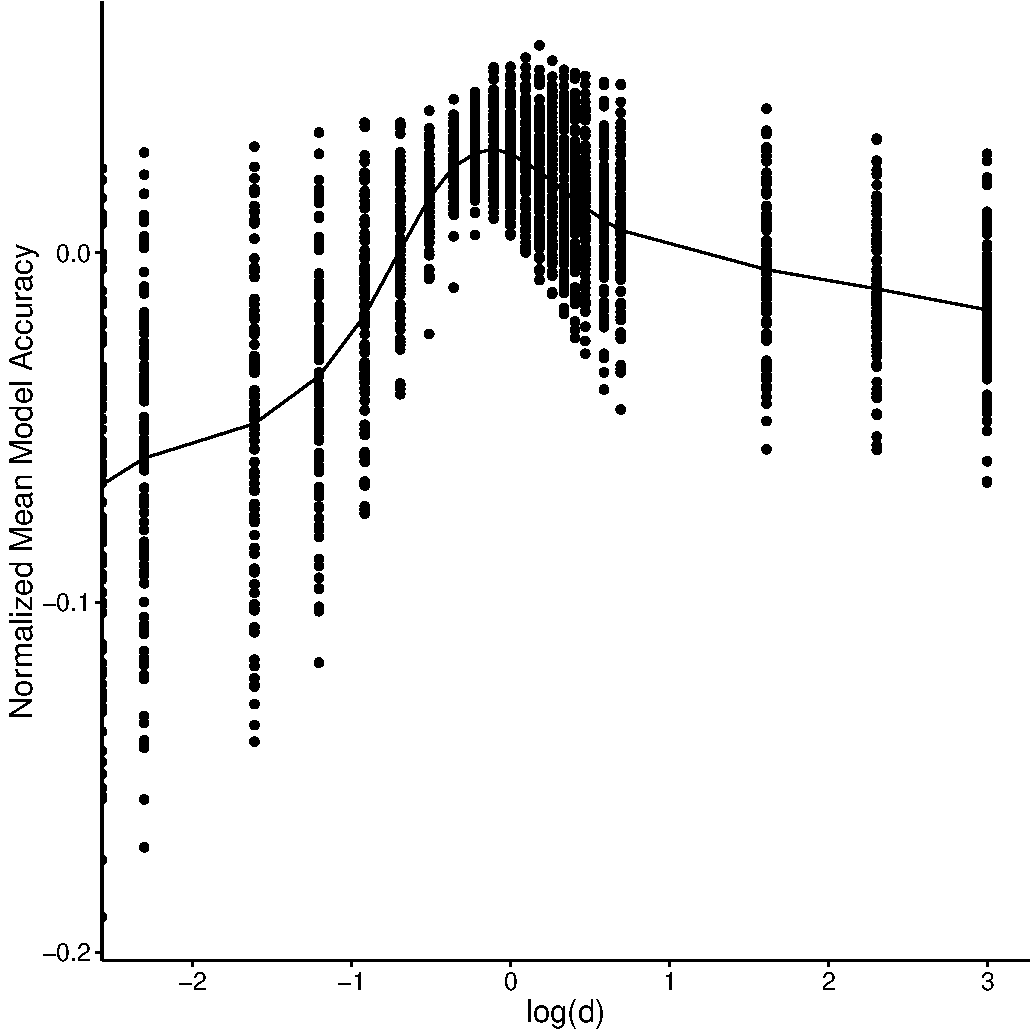
\includegraphics[width=5cm]{visNormMean-SOQgt500r2-topHashtagPostPriorStd-crop.pdf}}
    \hfill
    \subfigure[][Optimized learning form]{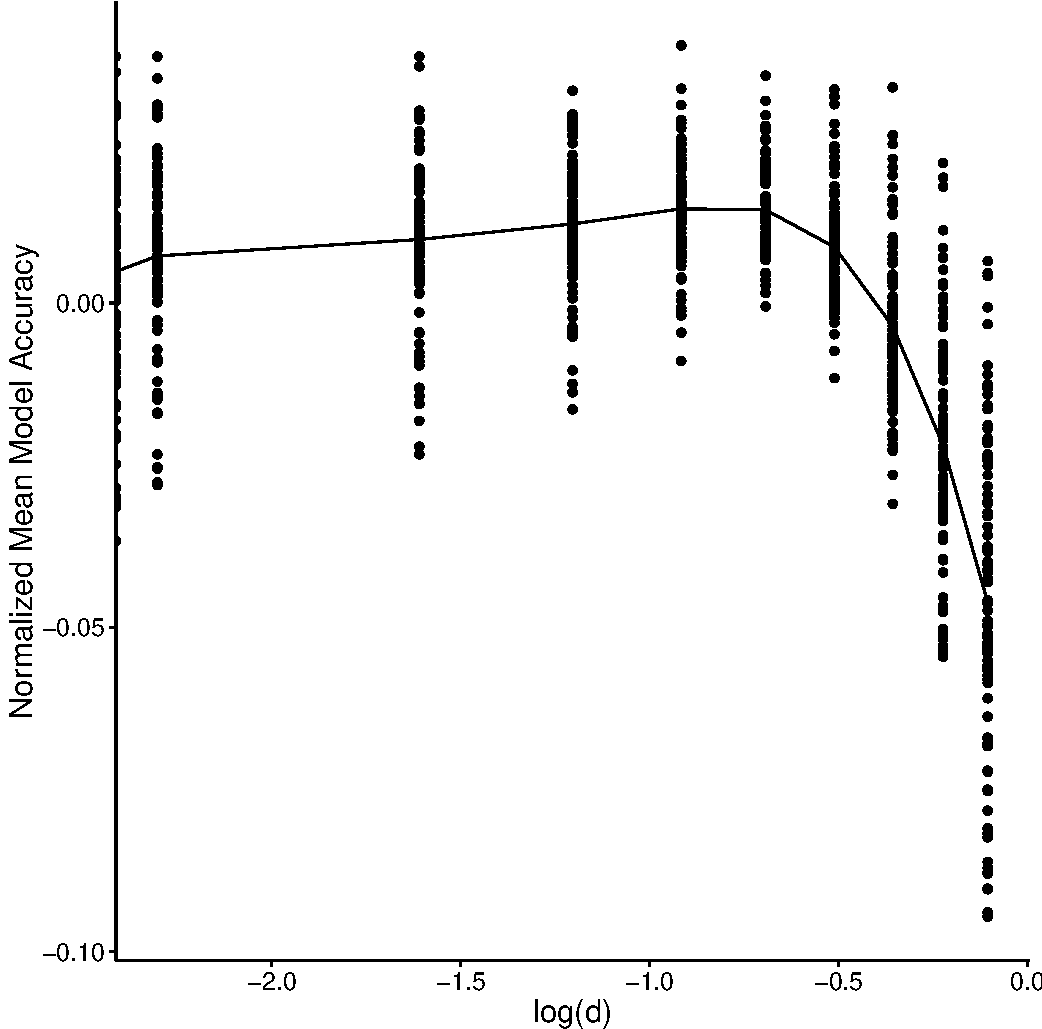
\includegraphics[width=5cm]{visNormMean-SOQgt500r2-topHashtagPostPriorOL2-crop.pdf}}
    \hfill
    \subfigure[][Hybrid form]{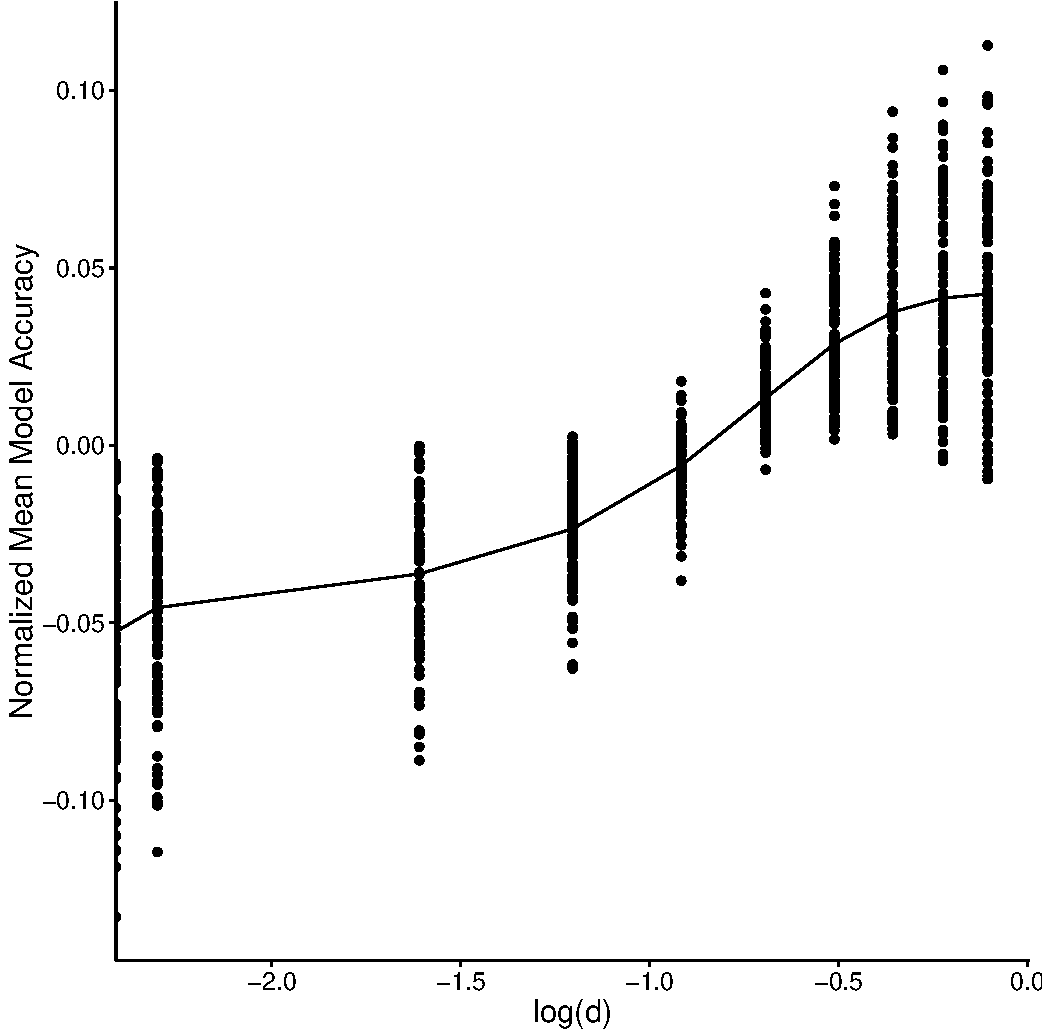
\includegraphics[width=5cm]{visNormMean-SOQgt500r2-topHashtagPostPriorHybrid10-crop.pdf}}
    \caption{
    Model performance for a single dataset slice for StackOverflow.
    This includes model accuracy as a function of decay rate value for each user in the dataset slice.
    Model accuracy is shown for the standard form of base-level activation ($B_{i}$), the optimized learning form, and the hybrid form when k=10.
  }
    \label{figPriorSOQSliceDsStd}
  }%

\end{figure}

\begin{figure}[!htbp]
  {%
    \setlength{\fboxsep}{0pt}%
    \setlength{\fboxrule}{1pt}%
    \hfill
    \subfigure[][Standard form]{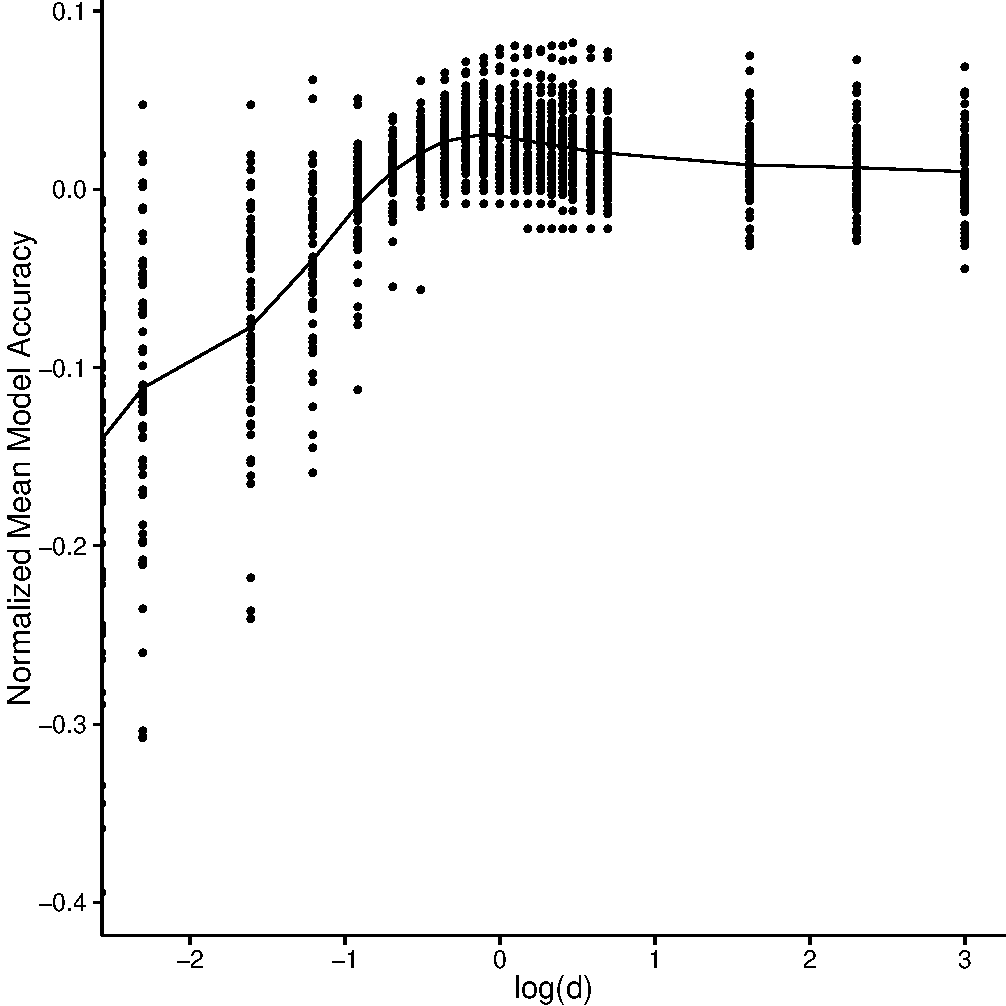
\includegraphics[width=5cm]{visNormMean-TFollowgt10Mr2-topHashtagPostPriorStd-crop.pdf}}
    \hfill
    \subfigure[][Optimized learning form]{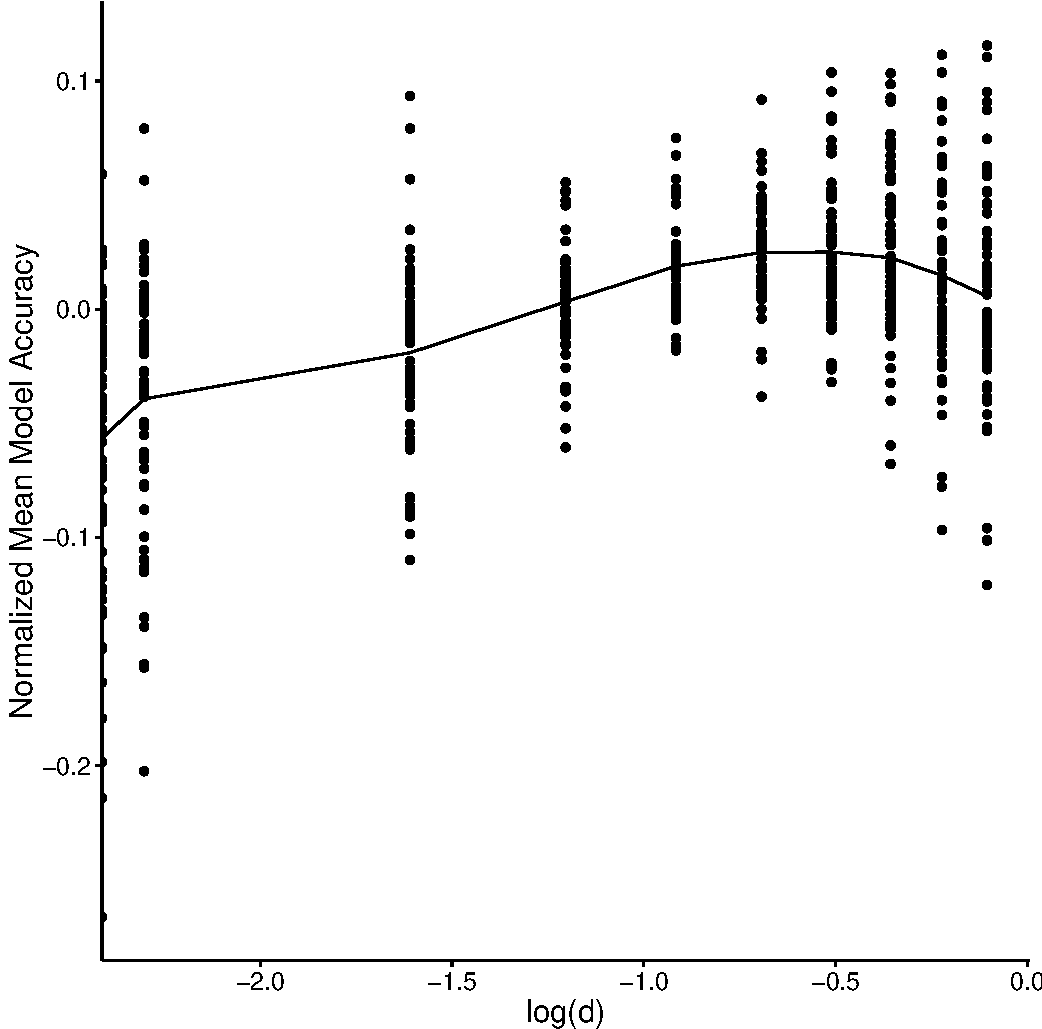
\includegraphics[width=5cm]{visNormMean-TFollowgt10Mr2-topHashtagPostPriorOL2-crop.pdf}}
    \hfill
    \subfigure[][Hybrid form]{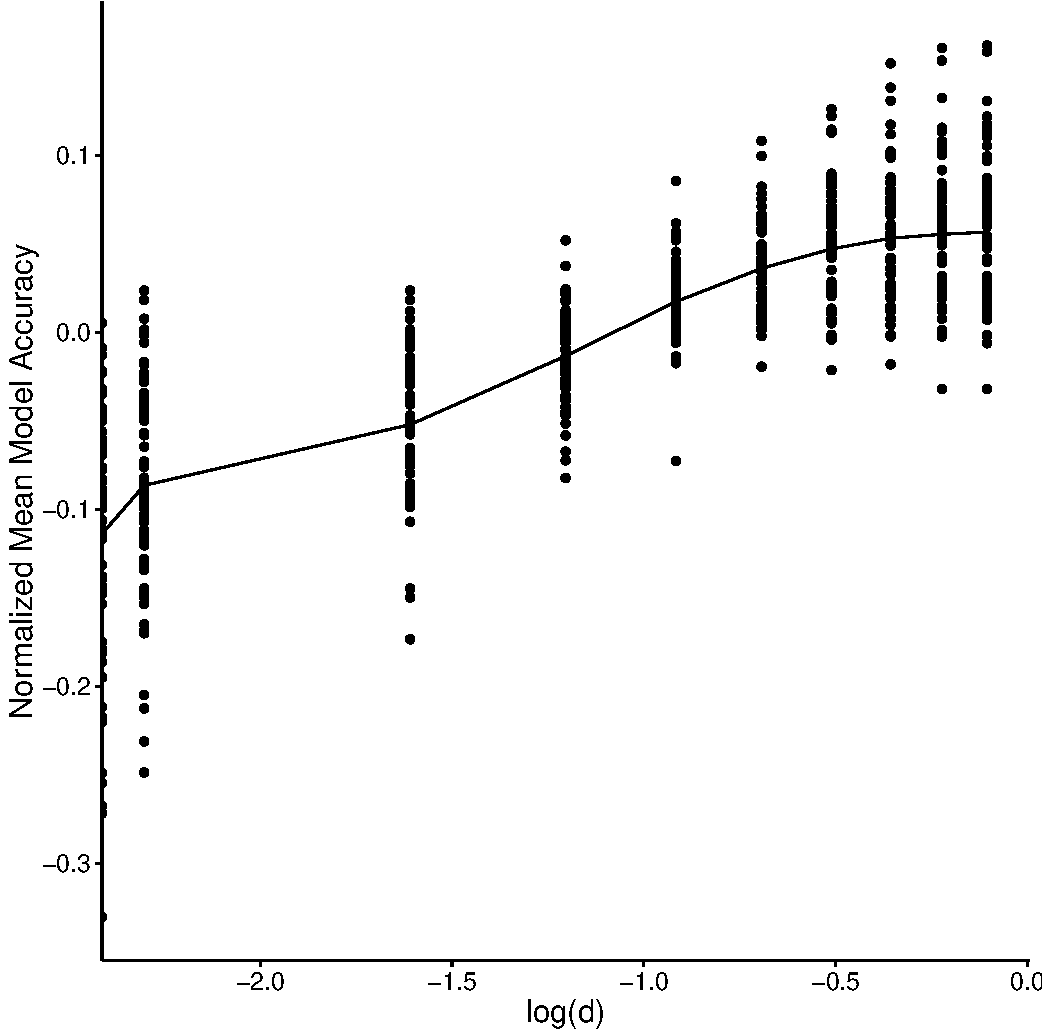
\includegraphics[width=5cm]{visNormMean-TFollowgt10Mr2-topHashtagPostPriorHybrid10-crop.pdf}}
    \caption{
      Model performance for a single dataset slice for Twitter.
      This includes model accuracy as a function of decay rate value for each user in the dataset slice.
    }
    \label{figPriorTwitterSliceDsStd}
  }%
\end{figure}

Model accuracies at each decay rate value for each user in the dataset slice are included in the plots.
Each user's mean accuracy was subtracted in order to compute a normalized mean for that user.
This was done so that the relative accuracy change for different decay rate values could be more easily visualized.
The plotting technique is a analogous to what is done when testing the main effect in a repeated measures design (i.e., each subject's mean score is subtracted).

One large effect in all of the plots is that there is an optimal decay rate value between 0 and 20 that produces the highest model accuracy.
For the standard $B_{i}$ equation, model accuracy for a pure frequency model ($d=0$) is also worse than using a pure recency model ($d=20$), particularly for Twitter.
It makes sense that a pure recency model for Twitter is relatively more accurate than for StackOverflow, as the hashtag lifetime for Twitter is much less than a tag for a programming language on StackOverflow.

When comparing the standard and optimized learning forms of the equation, it is apparent that a pure recency model does not work well for optimized learning.
The best-fit decay rate value for the optimized learning form is also not as clear and pronounced as it is for the standard form (less of a peak).
And the relative accuracy gained from using a pure frequency based model to a blend of frequency and recency is less for the optimized learning form than the standard form of $B_{i}$.
Finally, for the range defined for the hybrid form ($d < 1$), the standard and hybrid forms are shaped similarly across the decay rate values.

\subsubsection{Aggregate Model Performance}

Aggregate best-fit decay rates were computed by taking the median of all user's best-fit decay rate values across all dataset slices.
The median was used since there were users in the popular-users dataset that did not have enough observations to generate stable predictions, and best-fit decay rate values for these users could be as high as 20.
Using the median effectively trims these unstable values from the sample, without having to define a cut point for an outlier removal process.

Aggregate best-fit decay rate values for each model are included in Figure \ref{figPriorDecay}.
Decay rate values that produced the most accurate model performance are lower for the optimized learning form (\num{.43}) of $B_{i}$ compared to both the standard form (\num{.80}) and hybrid form (\num{.80} for all $k$).
The optimal values for optimized learning are near \num{0.5}, which lines up with default value used in ACT-R.

\begin{figure}[!htbp]
  \scalebox{.8}{\resizebox{\linewidth}{!}{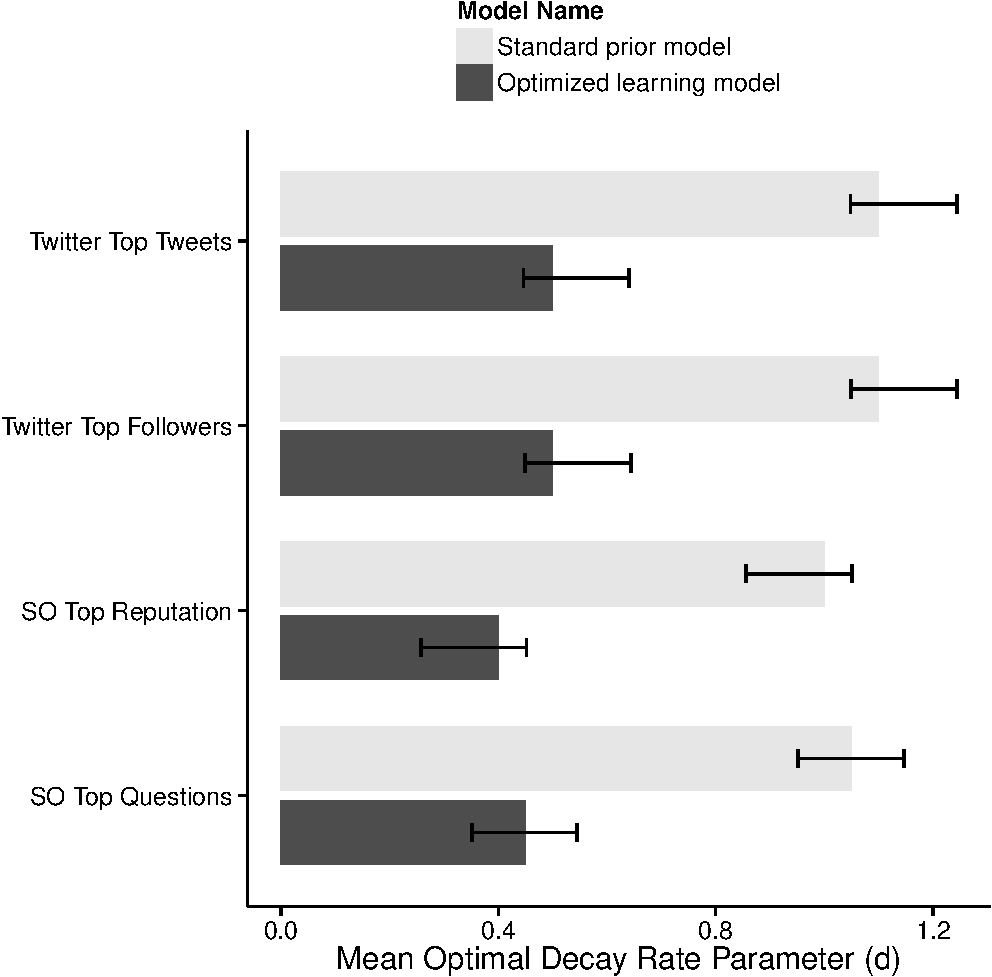
\includegraphics{compareMeanDV-d--crop.pdf}}}
  \caption{
  Overall best-fit decay rate for StackOverflow and Twitter.
  Results are shown for the two Twitter and StackOverflow (SO) popular-users datasets.
  Error bars represent the 95\% bootstrapped confidence interval for the median.
}
  \label{figPriorDecay}
\end{figure}

\FloatBarrier

Finally, model accuracy was analyzed across all dataset slices for StackOverflow and Twitter.
This was done by examining model accuracy at a specific decay rate value for each model.
Accuracy was assessed at each model's previously-determined best-fit values (\num{.43}, \num{.80}, and \num{.80} for the optimized learning, standard form, and hybrid form) and additionally the standard form's default value (\num{0.5}).
Since decay rate values were explored at \num{0.1} increments between the 0 and 1 range, the decay rate values used to examine model accuracy were rounded to the nearest decay rate value that was included in the run.
Consequently, a best-fit value of \num{.4} was used for the optimized learning model instead of the \num{.43} average found from the dataset slices.
Aggregate accuracy was computed by taking the mean of every user's model accuracy across all users in all dataset slices.


Accuracy for both sites is included in Figure \ref{figPriorAcc}. 
Accuracy for the standard form is higher than the optimized learning form (\numNoZero{.33} vs. \numNoZero{.28}, \myCI{.034}{.032}{.036}{3603}).
This makes sense given that the standard form does not assume equal presentation rate for each chunk, and hashtags on Twitter in particular show trends of high rate of use and then shift to low rate of use. 
The standard form of $B_{i}$ is able to more accurately account for these dynamics.

\begin{figure}[!htbp]
  \scalebox{.8}{\resizebox{\linewidth}{!}{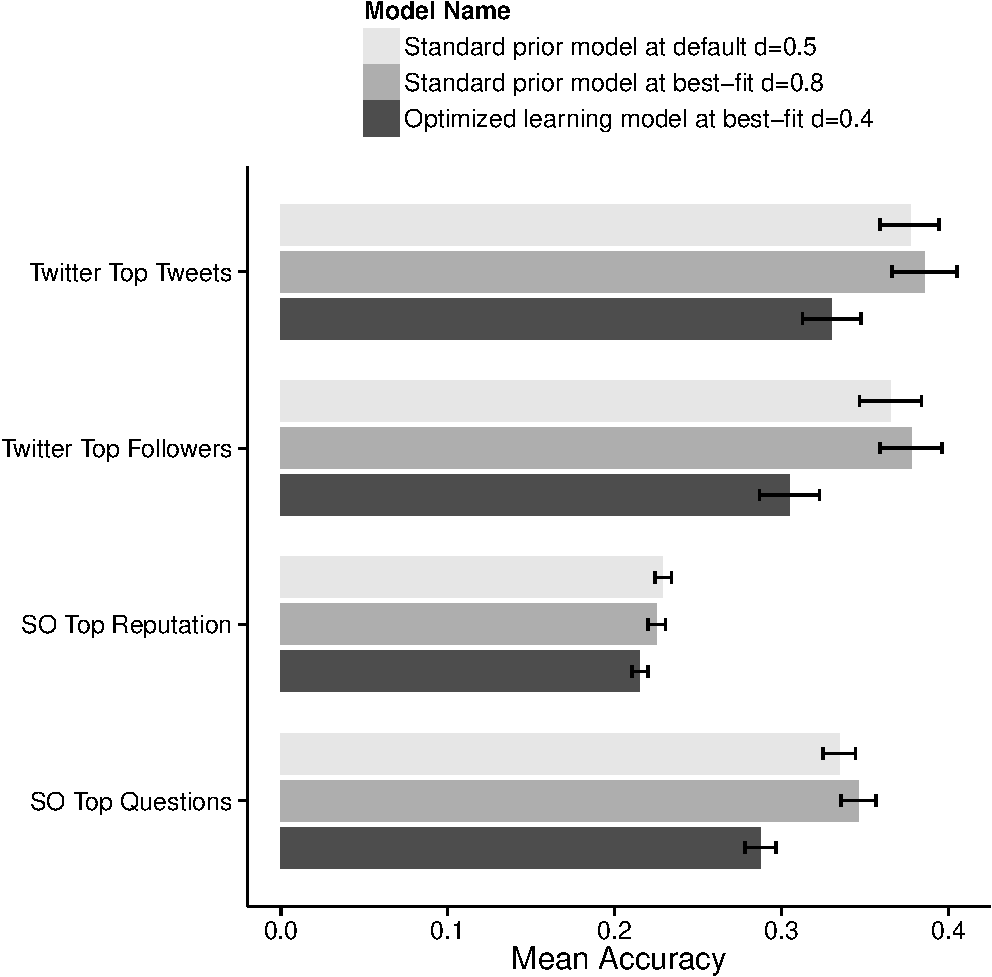
\includegraphics{compareMeanDV-acc--crop.pdf}}}
  \caption{
    Overall model accuracy for StackOverflow and Twitter at optimal decay rate values.
    All error bars are the 95\% bootstrapped confidence interval for the mean. 
  }
  \label{figPriorAcc}
\end{figure}

Accuracy for the hybrid form for the largest $k$ ($k=10$) is slightly higher than the smallest $k$ ($k=1$) (\numNoZero{.334} vs. \numNoZero{.329} \myCI{.0026}{.0023}{.0029}{3608}).
However accuracy cannot be distinguished between the hybrid form with the largest $k$ and the standard form (\numNoZero{.334} vs. \numNoZero{.334} \myCI{.0000}{-.0000}{.0001}{3609}).
This indicates that for the datasets analyzed in this study the hybrid form with $k=10$ is a suitable replacement to the standard form (produces the same results) and uses less computational resources than the standard form. 

ACT-R sets the default decay rate value to \num{0.5}, and the best-fit value for the standard form is higher (\num{0.8}) for these datasets.
The figure shows that although model accuracy does slightly improve (\num{0.325} to \num{0.335} \myCI{.0029}{.0022}{.0036}{3609}) for the standard form when increasing the decay rate parameter from \num{0.5} to the optimal value,
that percentage improvement is not as large (\num{0.28} to \num{0.33}) as the improvement gained from using the standard form compared to the optimized learning form.
Nonetheless, model accuracy is highest when both the standard form is used and the decay rate value is increased. 

\subsection{Discussion}

Given the large tag space used by post authors on StackOverflow and Twitter, it was surprising that model performance is respectable even when only past tag history and no context is used.
This speaks to the importance of taking into account overall past tagging history, and ensuring that the prior component of activation for each tag is customized to each user's specific past tagging history.

Also apparent for these datasets is that the optimized learning form of $B_{i}$ is not as accurate as the standard form.
Further, for the optimized learning form there is not much difference between using a pure frequency-based model and a model where frequency and recency are optimally blended.
This makes sense given that the optimized learning equation in Table \ref{tabACTRBLLModel} collapses to a pure frequency model as the amount of time since the presentation of the first recorded chunk instance increases,
and also since the timespan of recorded tag use for StackOverflow and Twitter is large (years).

However the hybrid form with a reasonable $k$ is just as accurate as the standard form.
This is due to the fact that the majority of change in activation for a chunk occurs in the short period of time after the presentation of the chunk (a property of a power law distribution).
Once a chunk's presentations decay to the flat area of the power law distribution, not much change in activation for these presentations occurs, so they can be averaged and their presentation time can be discarded without much loss in fidelity.
Therefore if computational speed is a concern, one may wish to leverage the hybrid form instead of the standard form.
Although qualitatively the standard form produces the cleanest and most natural effect of decay rate on accuracy, as shown in Figure \ref{figPriorSOQSliceDsStd}.
It also does not have a bifurcation at $k=1$.
Consequently, if one is a purist and computational speed is less of a concern, one may still wish to use the standard form over the hybrid form.

\section{Combining Predictors}

The declarative memory models analyzed for this research consist of two main components: past behavior and context.
Past tag use was isolated in the first section to see how well ACT-R's prior component of declarative memory (i.e., base-level learning) fits each user's tag use over time.
For the next section the past behavior and context declarative memory components were combined as well as looked at in isolation.

This section will examine how model accuracy is influenced by four architectural concerns:
method of handling stop words, influence of dataset size, method of combining prior and context, and word order.
These particular architectural concerns were examined for the following reasons:
During exploratory evaluation, model accuracy seemed to be highly sensitive to the method of dealing with the commonly-used stop words, so several different methods were examined in more detail.
Due to research from \textcite{Budiu2007} and \textcite{Recchia2010}, model accuracy for the Bayesian and vector-based models is influenced by the number of documents in the dataset,
so the effect of dataset size on accuracy was examined in more detail.
One of the primary goals of this research is to identify the best method to combine the model term for past user behavior with the context term for the random permutation model,
so two different ways to add the model terms were tested.
Finally, previous research has shown that including word order in the vector-based models improves performance \parencites{Jones2007, Sahlgren2008},
so word order was also examined to see if the effect could be replicated and also to measure the overall importance of word order on model accuracy relative to other architectural manipulations.

\subsection{Overall Method}

\subsubsection{Logistic Regression}

In order to best combine these predictors, a logistic regression statistical technique similar to \textcite{Stanley2013} was used to determine the most optimal weights for each term.
When a user creates a tag for a post, a retrieval request for the model is made.
For each request, the model returns a set of tags (all tags that have been observed for that user in the past) and activations associated with each tag.
An activation value is computed for each model component (e.g., prior tag use, context) for each tag.
These values are recorded, and tag instances that match what the author actually tagged are marked as a 1, while all others are marked with a 0.
When an author used multiple tags for a post, multiple 1s are marked for that post.
This process is repeated across all posts where a user chooses a tag, and across all users in the dataset.
Once all of the results are aggregated, a logistic regression is run where the optimal weights for each model component are found that maximize the model's ability to correctly label tags as 0 or 1 based on total activation.

Model accuracy was evaluated by rank ordering all recorded tags by model activation using the optimal weights,
asking the model to tag the top N posts with a 1 (where N is the total number of recorded tagging instances in the dataset sample),
and then comparing the model's chosen tags with the used tags for each post (i.e., looking at the ``hits'').
This is equivalent to throttling the threshold in the logistic regression such that the total number of observations labeled as a 1 match the total number of recorded instances of tagging in the dataset.

\subsubsection{Adding Offset Term}

This logistic regression method is a computationally efficient way to find the optimal weights for the predictors.
However, when the regression can not be constrained to label a specific number of 1s for each observation (as is the case here), to be used properly an offset term must be added as an additional model predictor.
The offset term keeps the activation for the small number of top tags for each post equal across posts.
This ensures that the logistic regression only labels a few 1s for each post.

A simplified version of \textcite{Stanley2013}'s method was used for this research.
Instead of subtracting the mean total activation for the top 5 tags for each post, the process is done in isolation for each model component.
For the prior component for example, the activation value used in the logistic regression is the prior activation with the mean of the top 5 prior activations subtracted from this value.
The same process is used for the context component.
Decoupling the offset term and computing an offset for each model component in isolation means that an iterative approach was no longer necessary,
since the optimal weights of the terms are no longer needed when computing the offset.

\subsubsection{Datasets}

Model accuracy was tested on the popular-hashtags dataset for Twitter and a random sample of posts across the entire StackOverflow dataset.
For each of the four Twitter popular-hashtags datasets, model retrievals were done across 15 runs and 500 posts within each run.
For the StackOverflow randomly-sampled dataset, 5 runs of 100 posts were used,
since the results for StackOverflow were more stable and retrievals took more wall-clock time for this dataset due to the size of the co-occurrence matrix.
All runs contained different posts, and all posts used for runs were not used to generate the co-occurrence matrix for the two retrieval models.

\subsubsection{Computing Priors}

For each randomly-sampled post for StackOverflow, the prior activation is based on that user's prior tagging history, and not on any global prior of specific tag frequency across users.
This was done so that the prior component used for StackOverflow for both the popular-users and randomly-sampled datasets was the same.

However, a custom user prior for the Twitter popular-hashtags dataset could not be used, since the entire Twitter dataset could not be downloaded, so the history of every user in the popular-hashtags dataset could not be collected.
Instead, the global prior tag history for all users in the Twitter popular-hashtags dataset was used to compute prior activation values for each tag.

\subsubsection{Co-occurrence Matrices}

The context component for both the random permutation and Bayesian model was based on the same co-occurrence matrix of words and observed tags.
Different size matrices were analyzed, ranging from \num{1000}, \num{10000}, \num{100000}, \num{1000000}, and \num{3000000} posts.
The matrix for \num{3000000} posts was only used for Twitter, since the number of words in a StackOverflow post is much higher than Twitter on average,
and the space and computational time required when using a co-occurrence matrix of \num{3000000} posts for StackOverflow was too large. 

\subsection{Stop Words}

The method of handling stop words has been shown to influence model accuracy \parencite{Sahlgren2008,Stanley2013,Jones2007}, so this was the first architectural concern that was examined.
``Stop words'' (e.g., ``the,'' ``a,'' ``or'') are commonly used words that co-occur with all tags (i.e., have little to no discriminating power).
\textcite{Sahlgren2008} looked at several ways to handle the commonly-occurring stop words for the random permutation model:
A data-driven frequency-filtering approach was tried, along with using a previously-generated stoplist, and no stop word removal at all.
However, \citeauthor{Sahlgren2008} did not try to weight the stop words and only tried methods to remove them.

\textcite{Stanley2013} used the entropy weighting technique recommended in \textcite{Dumais1991} for the StackOverflow dataset.
The technique is formally described in Table \ref{tabModACTRModel} and uses information theory to determine the amount of predictive information contained in each word.
Words that are often used with a small number of tags have high information content while words used often across all tags carry low information content.
This method maps cleanly to the ACT-R DM theory by modifying each word's attentional weight ($W_{j}$) parameter.

\subsubsection{Method}

The runs from the Twitter popular-hashtags and StackOverflow randomly-sampled datasets were used for the analysis.
Both the random permutation and Bayesian models were tested.
Activations for context were computed by using five different methods to handle stop words:
The two removal methods used in \textcite{Sahlgren2008}
(i.e., removal based on frequency, removal based on the pre-determined 571-word Cornell SMART stoplist: \noparencite{Salton1988}),
the entropy-weighting method used in \textcite{Stanley2013},
combining the entropy-weighting and frequency-filtering methods,
and no removal or weighting of stop words.

\paragraph{Determining Frequency Cutoff}

A cutoff point must be identified and used in order to remove the high-frequency words.
\textcite{Sahlgren2008} used a cutoff where words that occurred more than \num{15000} times were removed.
Since the StackOverflow and Twitter datasets are much larger than the datasets used by \citeauthor{Sahlgren2008}, the same cutoff could not be used.

The ideal cutoff was determined by choosing the value where the standard deviation of the counts for each word for each of the tags were all relatively small.
The plots for the standard deviations across tags that were used to identify the cutoff for StackOverflow and Twitter are shown in Figures \ref{figContextCutoffSO} and \ref{figContextCutoffT}.

\begin{figure}[!htbp]
  \scalebox{.8}{\resizebox{\linewidth}{!}{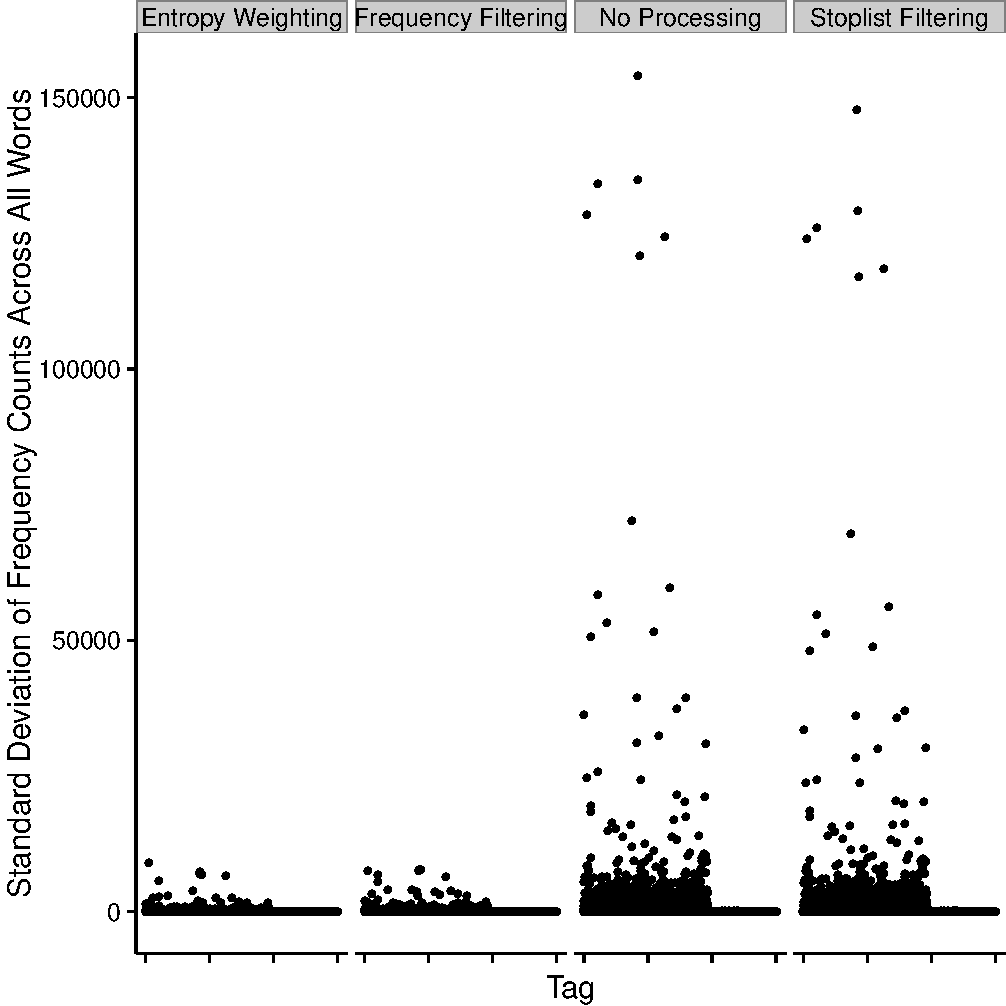
\includegraphics{memMatSO-crop.pdf}}}
  \caption{
    Variance in observation counts of words for each tag for StackOverflow.
    Plots are shown for the four different methods for handling stop words.
    Each plot contains the standard deviation of the total counts for each word in context as a function of hashtag.
    High values mean that there are context words for a hashtag that have a high number of counts relative to the counts for all other context words for that hashtag.
  }
  \label{figContextCutoffSO}
\end{figure}

\begin{figure}[!htbp]
  \scalebox{.8}{\resizebox{\linewidth}{!}{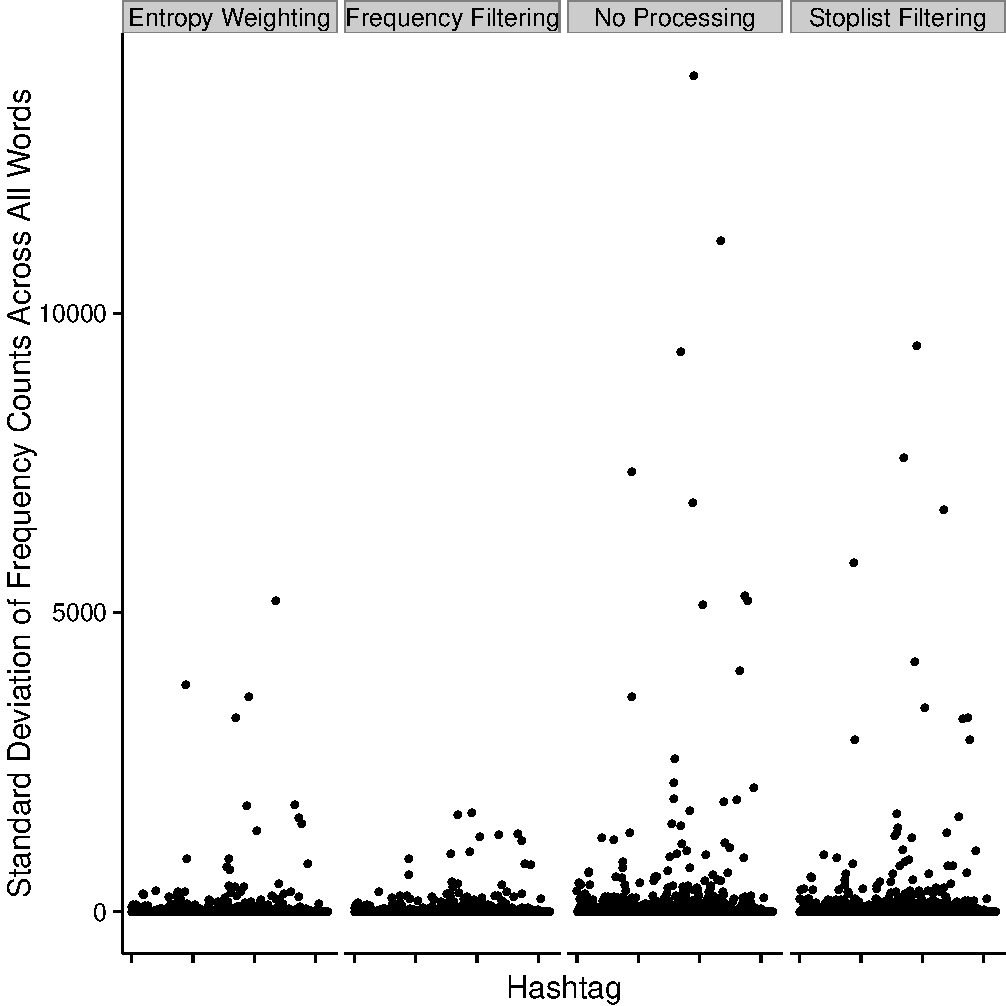
\includegraphics{memMatT-crop.pdf}}}
  \caption{
    Variance in observation counts of words for each tag for Twitter.
  }
  \label{figContextCutoffT}
\end{figure}

The ``no processing'' plot shows the size of the spikes when high-frequency words are not removed.
The entropy plot shows how the size decreases by more than an order of magnitude after the entropy weighting measure is used.
The cutoff for the frequency plot was chosen such that the plot looks similar to the entropy plot, with spikes around the same size.
The cutoff that produced the frequency plots in Figures \ref{figContextCutoffSO} and \ref{figContextCutoffT} is where a word represents more than \num{.04}\% of total occurrences in the dataset.

\subsubsection{Results for the Random Permutation Model}

Plots for the three methods of handling stop words for the random permutation model on the StackOverflow dataset are shown in Figure \ref{figContextStopRPSO}.
In the plot, if the model name includes ``full'' then all model components are included.
When the model components are enumerated, then at least one of the components is left out.
For example, the ``standard prior model relaxed across posts'' means that only the prior model component was used when determining activation. 
As another example, ``RP only title with freq'' means that only the title context component of the random permutation model was used, and that stop words were handled using the frequency filtering technique.

\begin{figure}[!htbp]
  \scalebox{.8}{\resizebox{\linewidth}{!}{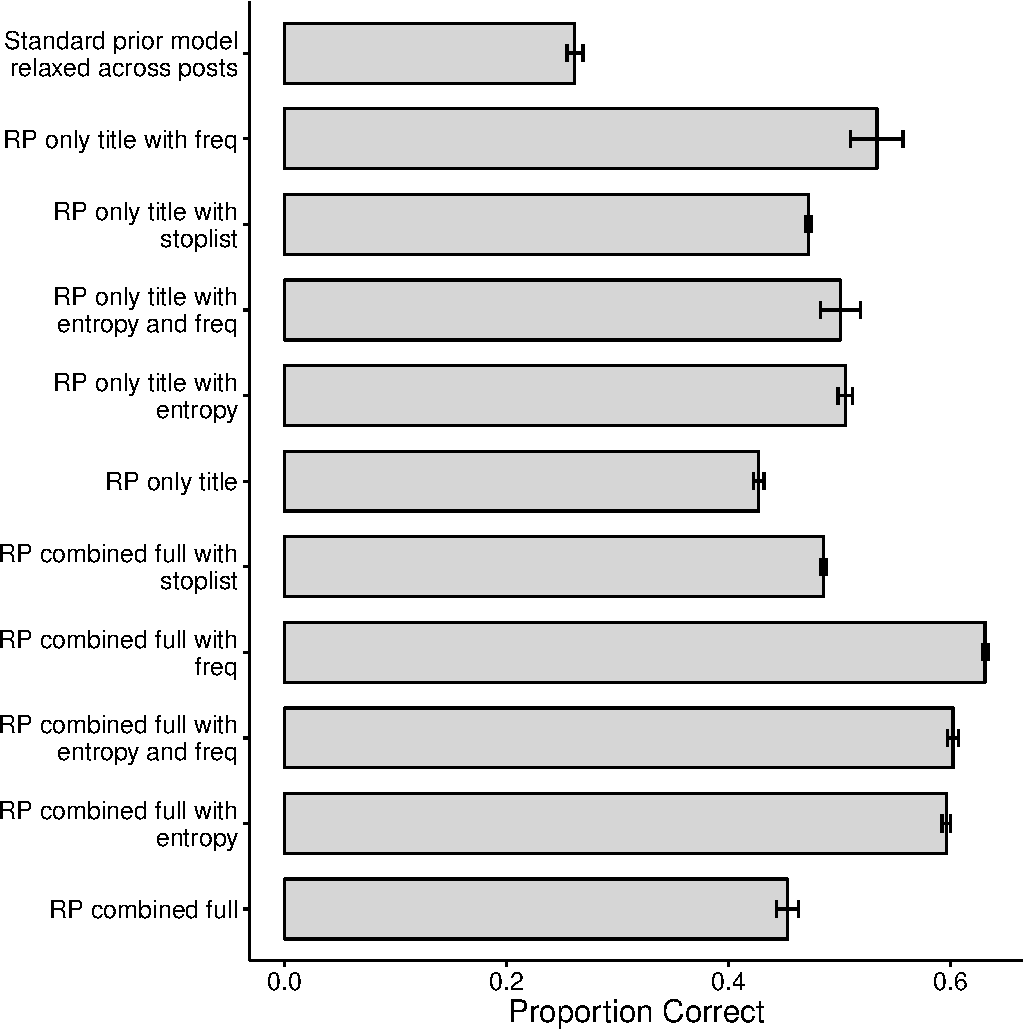
\includegraphics{compareMeanDV-acc-allWeightingsSOPerm-crop.pdf}}}
  \caption{
    Stop-word techniques for the random permutation model for StackOverflow.
    The five methods for handling stop words are shown both for the title model component in isolation and the full model.
    ``Stoplist'', ``freq'', ``entropy'' are the stoplist removal method, removal based on frequency count, and weighting based entropy metric.
    All error bars are the 95\% bootstrapped confidence interval for the mean. 
}
  \label{figContextStopRPSO}
\end{figure}

The results show that model accuracy improves if stop words are handled in any of the three ways (predefined stoplist filtering, entropy weighting, and frequency filtering).
Using a predefined stoplist makes the smallest improvement (\numNoZero{.45} to \numNoZero{.49}, \myCI{.032}{.018}{.047}{5})
while the entropy (\numNoZero{.45} to \numNoZero{.60}, \myCI{.143}{.123}{.163}{5}) and frequency (\numNoZero{.45} to \numNoZero{.63}, \myCI{.178}{.164}{.192}{5}) techniques improve performance the most,
and frequency shows a slight edge over entropy.
However, using the frequency-filtering technique produces more noise in accuracy measurements compared to the other techniques, at least when tested on words in the title of StackOverflow posts.

The three stop word techniques were then tested for the random permutation model on the Twitter dataset, and the results are depicted in Figure \ref{figContextStopRPT}.
For the random permutation model for Twitter, the entropy weighting technique is the best method for handling stop words (\numNoZero{.25} to \numNoZero{.26}, \myCI{.013}{.011}{.015}{60}).
Removing stop-words based on a predetermined list actually decreases accuracy (\numNoZero{.25} to \numNoZero{.23}, \myCI{-.017}{-.015}{-.019}{60}),
and using data-driven frequency filtering has only a small to no effect (\numNoZero{.25} to \numNoZero{.25}, \myCI{.00}{-.003}{.002}{60}).

\begin{figure}[!htbp]
  \scalebox{.8}{\resizebox{\linewidth}{!}{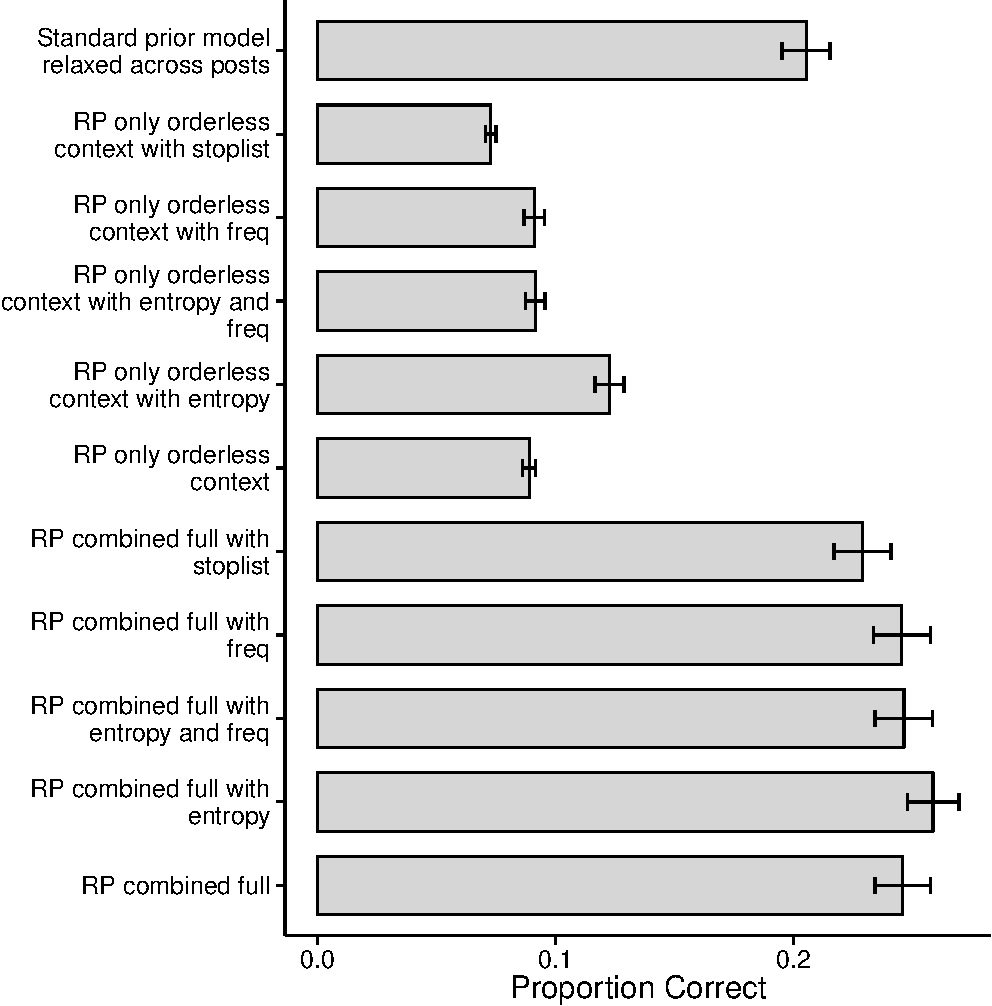
\includegraphics{compareMeanDV-acc-allWeightingsTPerm-crop.pdf}}}
  \caption{
  Stop-word techniques for the random permutation model for Twitter.
  The five methods for handling stop words are shown both for the context model component (i.e., no prior term) and the full model.
  All error bars are the 95\% bootstrapped confidence interval for the mean. 
}
  \label{figContextStopRPT}
\end{figure}

\subsubsection{Results for the Bayesian Model}

Since accuracy measurements when using a predetermined list to remove stop words for the random permutation model were much worse than the frequency and entropy methods, this method was not examined for the Bayesian model.
The results for the frequency and entropy techniques for the Bayesian model on the StackOverflow dataset are depicted in Figure \ref{figContextStopBSO}.

\begin{figure}[!htbp]
  \scalebox{.8}{\resizebox{\linewidth}{!}{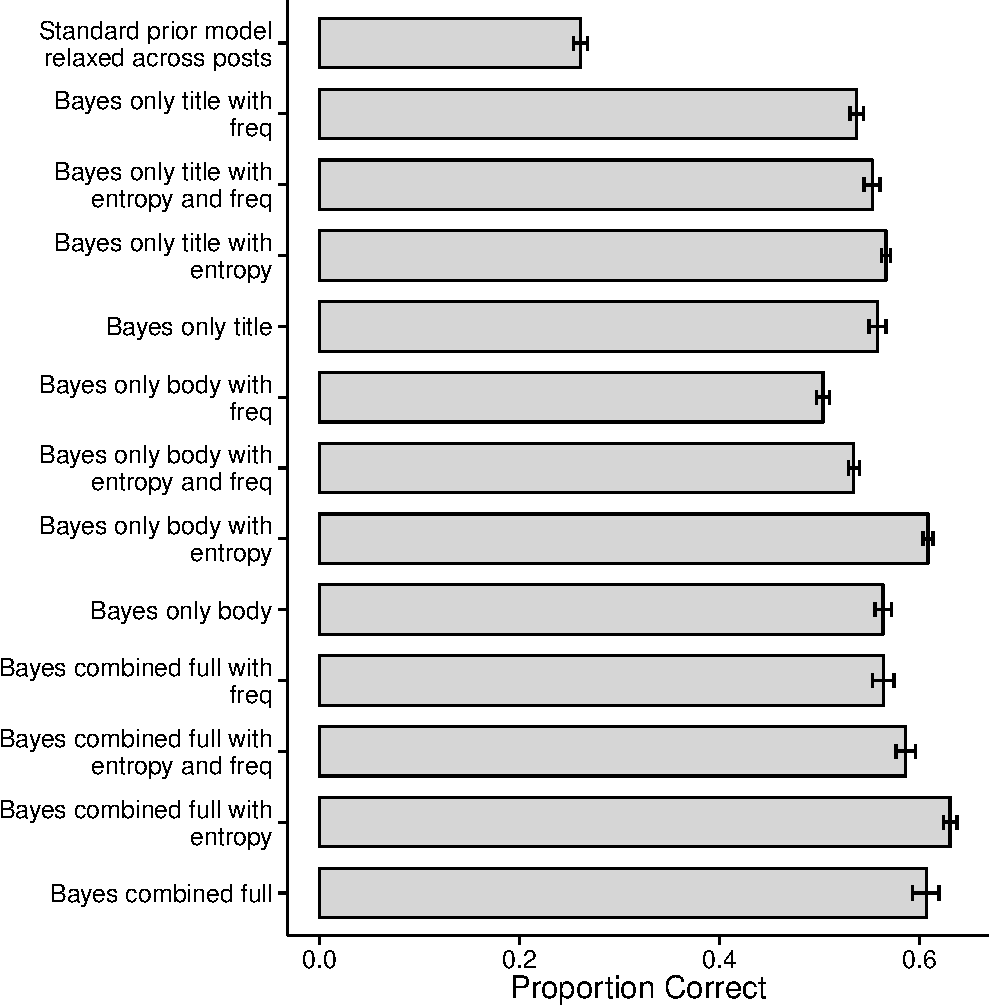
\includegraphics{compareMeanDV-acc-allWeightingsSOSji-crop.pdf}}}
  \caption{
  Stop-word techniques for the Bayesian model for StackOverflow
  All error bars are the 95\% bootstrapped confidence interval for the mean. 
}
  \label{figContextStopBSO}
\end{figure}

The results show that entropy weighting produces the most accurate results (\numNoZero{.61} to \numNoZero{.63}, \myCI{.024}{.011}{.037}{5}).
Also, accuracy actually decreases when using frequency filtering compared to no filtering (\numNoZero{.61} to \numNoZero{.56}, \myCI{-.043}{-.030}{-.057}{5}) for the Bayesian model.
So entropy weighting is the clear winner in this case.

Similar results are found when the Bayesian model is tested on the Twitter dataset.
Figure \ref{figContextStopBT} shows that entropy weighting is again the best performer (\numNoZero{.29} to \numNoZero{.32}, \myCI{.028}{.024}{.031}{60}),
and frequency filtering decreases performance relative to no filtering (\numNoZero{.29} to \numNoZero{.28}, \myCI{-.017}{-.015}{-.019}{60}).

\begin{figure}[!htbp]
  \scalebox{.8}{\resizebox{\linewidth}{!}{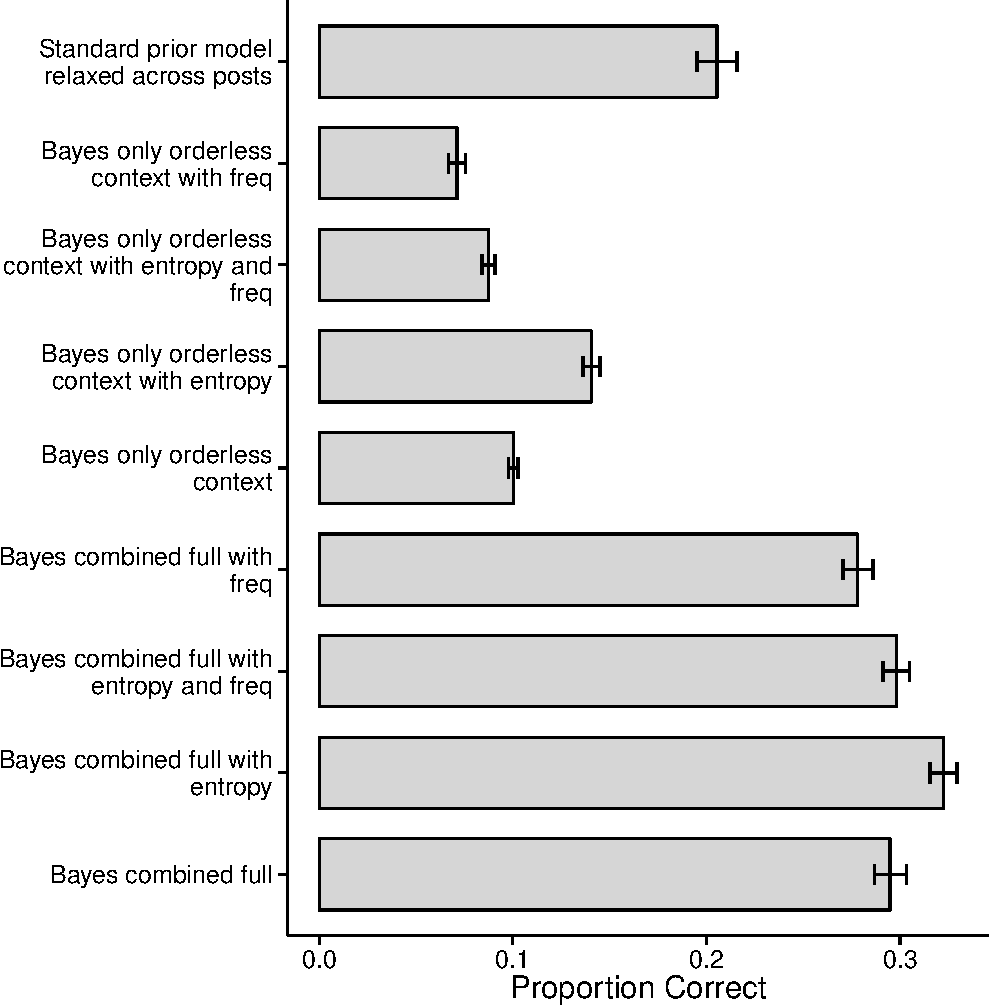
\includegraphics{compareMeanDV-acc-allWeightingsTSji-crop.pdf}}}
  \caption{
  Stop-word techniques for the Bayesian model for Twitter
  All error bars are the 95\% bootstrapped confidence interval for the mean. 
}
  \label{figContextStopBT}
\end{figure}

\subsubsection{Discussion}

One result that should not be overlooked is how poorly using a predetermined stoplist performed when compared to the two data-driven frequency and entropy approaches.
This is most likely because the StackOverflow and Twitter datasets are large and contain high-frequency words that are domain specific (e.g., emoticons) and are not included in the predetermined list.
This shows that data-driven techniques to identify stop words can be much more effective than using a predetermined list.

Another interesting result is how the Bayesian model actually performed worse when stop words were removed based on frequency compared to no stop word removal.
This was not the case for the random permutation model in this study, was not the case when \textcite{Sahlgren2008} used frequency filtering on the random permutation model,
and is most likely never the case for the random permutation model.
Model accuracy most likely decreases for the Bayesian model because this model already has a normalization component built in that the random permutation model does not have.
When computing activation for the random permutation model, the correlation is calculated directly on a matrix of counts of co-occurrences for words and tags.
For the Bayesian model this count matrix is converted to a log-odds ($S_{ji}$) matrix,
where both the number of observations for the word and the tag are normalized when computing the value for each cell (see the $S_{ji}$ computation in Table \ref{tabModACTRModel}).
Therefore, it is likely the case that a form of frequency attenuation is already built into the Bayesian model,
and adding a frequency filter on top of this does nothing to improve accuracy and only removes predictive information.

\textcite{Stanley2013} found that the entropy-weighting technique to attenuate stop words for the Bayesian model significantly improved model accuracy.
The same effect is found for the StackOverflow and Twitter datasets in this study.
Further, when this entropy-weighting technique is compared directly to the more common frequency-filtering technique, weighting by entropy produces more accurate results.
This was clearly the case for the Bayesian model.
Both frequency and entropy techniques performed equally for the random permutation model.
However, since the entropy-weighting technique is parameter-free and does not require a cutoff to tune, it is also a better choice for the random permutation model for these datasets.

\subsection{Corpus Size}

The number of documents used to build the co-occurrence matrix has been shown to influence model accuracy \parencite{Sahlgren2008}.
The default number of documents used to build the co-occurrence matrix was \num{1000000} for StackOverflow and \num{3000000} for Twitter.
In order to see how accuracy changed as function of corpus size, 
co-occurrence matrices for a range of smaller corpus sizes were built.

\subsubsection{Method}

For StackOverflow, the following number of posts were used to build separate co-occurrence matrices: \num{1000}, \num{10000}, \num{100000}, and the default \num{1000000}.
For Twitter, these matrix sizes were tested alongside the default \num{3000000}.
All runs from the four Twitter popular-hashtags datasets and the randomly-sampled StackOverflow dataset were used to test model accuracy.

\subsubsection{Results for StackOverflow}

Model accuracy as a function of co-occurrence matrix size for StackOverflow is depicted in Figure \ref{figContextDocumentSizeSO}.
Accuracy improves for both the Bayesian and random permutation models as the size of the documents used to generate the co-occurrence matrix increases.
However for the random permutation model, accuracy begins to plateau for the largest corpus size for all three tested versions. 
The Bayesian model does not plateau nearly as much and accuracy continues to improve even at the largest measured corpus size. 

\begin{figure}[!htbp]
  \scalebox{.8}{\resizebox{\linewidth}{!}{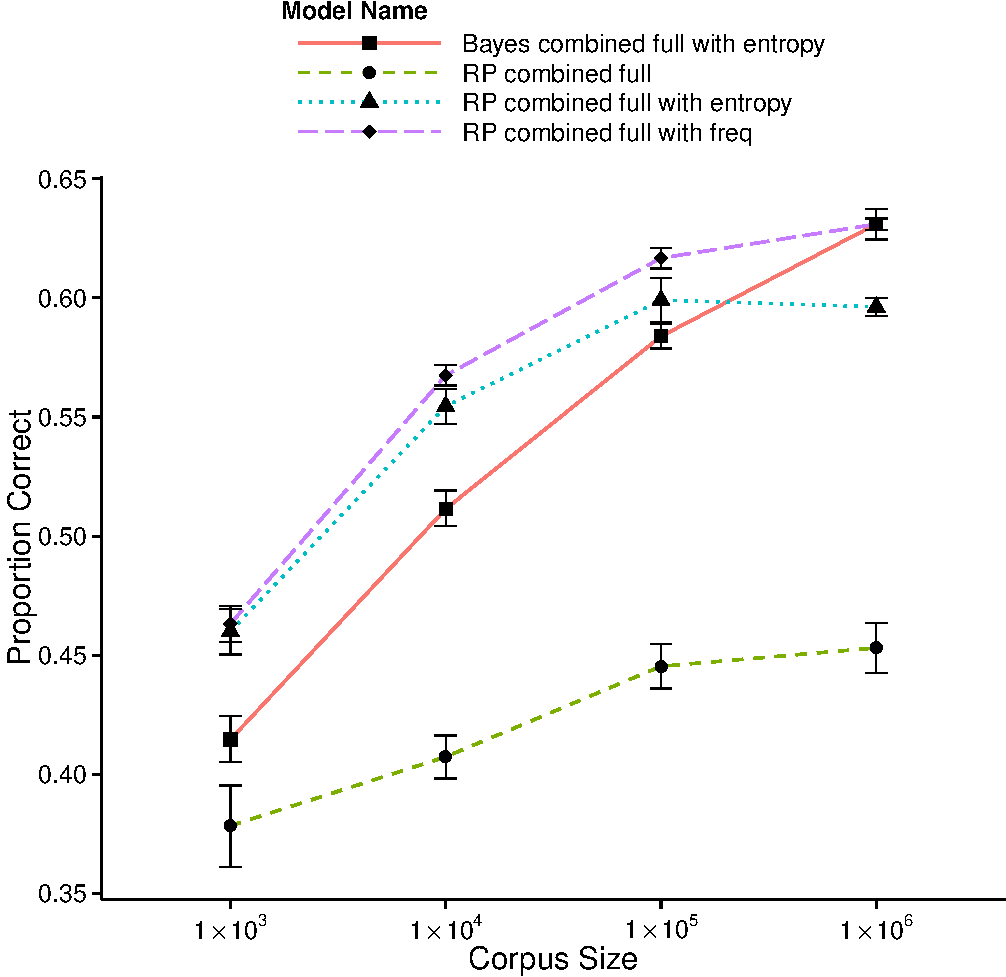
\includegraphics{compareMeanDV-acc-freqVsEntropyBySizeSO-crop.pdf}}}
  \caption{
    Effect of size of co-occurrence matrix for StackOverflow.
    Error bars represent the 95\% bootstrapped confidence interval for the mean model accuracy across all runs in dataset.
  }
  \label{figContextDocumentSizeSO}
\end{figure}

\subsubsection{Results for Twitter}

The overall trend of increasing accuracy with corpus size is present for Twitter as well.
Both entropy weighting and frequency filtering in Figure \ref{figContextDocumentSizeT} plateau for the random permutation model with increasing corpus size.
Once again, the Bayesian model continues to improve with corpus size.

\begin{figure}[!htbp]
  \scalebox{.8}{\resizebox{\linewidth}{!}{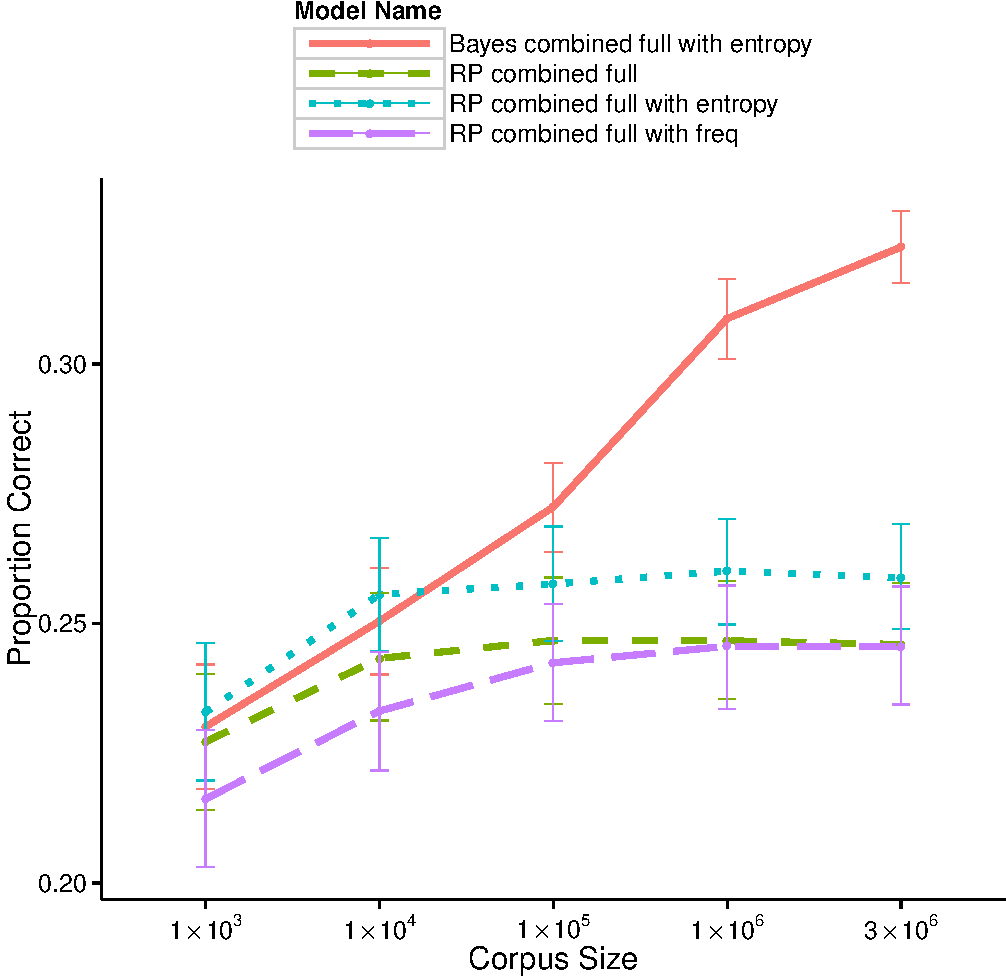
\includegraphics{compareMeanDV-acc-freqVsEntropyBySizeT-crop.pdf}}}
  \caption{
    Effect of size of co-occurrence matrix for Twitter.
    Error bars represent the 95\% bootstrapped confidence interval for the mean.
  }
  \label{figContextDocumentSizeT}
\end{figure}

\subsubsection{Discussion}

It is interesting to compare model accuracy between the Bayesian and random permutation model at the smallest and largest corpus sizes for both StackOverflow and Twitter.
At smaller corpus sizes, the random permutation model outperforms the Bayesian model (slightly for Twitter, dramatically for StackOverflow), and this performance difference diminishes as corpus size increases.
In other words, the Bayesian model needs larger co-occurrence matrices than the random permutation model to work properly.
As the size of the dataset increases, the compression may start to lose crucial information, and the uncompressed Bayesian model should be used.
As the size of the dataset decreases, the noise and crosstalk introduced by the compression for the random permutation model is actually beneficial, and the compressed random permutation model should be used. 
This noise is beneficial because it helps soften spurious $S_{ji}$ values when the counts for each individual cell in the co-occurrence matrix are still volatile, which happens at smaller corpus sizes.

This result has important implications.
The corpus size is rarely chosen, and more likely constrained by the number of documents in the dataset being studied.
If that dataset is relatively small, it may be better to use the compressed random permutation model than the Bayesian model, and vice-versa if the dataset is large.

However, corpus size is not the only factor that determines whether the Bayesian model or random permutation model will perform better.
This is because the number of observations used to generate the co-occurrence matrix is a function of four components:
corpus size, number of words in each document, total number of unique tags, and number of tags used per document.

The compressed random permutation model should perform better with smaller corpus sizes, less words per document, more unique tags, and fewer number of tags per post.
However, since there are so many factors that determine whether the Bayesian or random permutation model will perform better,
and only two different datasets were examined in this research,
it is difficult to make any specific recommendations as far as exact transition cut points (e.g., corpus size, words per document) where either the Bayesian or random permutation model should be used.
Also, it is likely that the specific domain being studied interacts with the factors already mentioned to determine which model is better for that domain.
Nevertheless, if a researcher is working in a domain with limited data (e.g., small corpus size, large tag space) that produces a sparse co-occurrence matrix,
then it may be worthwhile to experiment with using a compressed random permutation model instead of the full Bayesian model.
Also, newer models of $S_{ji}$ have been introduced that have a more local impact when a new chunk is observed \parencite{thomson2013constraining}.
It would also be interesting to see how these local models of $S_{ji}$ perform while varying the number of observed associations.

\subsection{Combining Prior and Context}

The activation value for the context component of the vector-based model is a correlation, ranging from zero to one.
This is not a log-odds value.
For the previous results, prior and context for the random permutation model were combined by simply adding the terms.
However, this means that ACT-R's prior base-level learning component (which is a log-odds value) is added to a correlation value, which may not be mathematically appropriate.
As a third architectural concern, another method to combine the prior and context components for the random permutation model was explored.

\subsubsection{Method}

For a given retrieval, the random permutation model returns a set of activations that are correlation values for each of the tags.
Instead of simply adding this correlation value to the prior model term, it may be more appropriate to convert the correlation value to a log-odds value first, and then add this context term to the log-odds prior term.
So a method was created to convert a distribution of correlations to a distribution of log-odds values.
To do this, the one-tailed cumulative distribution function value for each correlation was computed.
That probability was then converted to a log-odds value in the usual way. 

This technique has a few advantages: 
It is simple and computationally cheap.
Also, it behaves properly at specific points in the distribution.
For example, if the conversion is performed on the mean correlation value in the set, the result is a log-odds value of zero.
This makes sense given that log odds can be interpreted as the amount of odds information (positive or negative) that should be adjusted to the prior log odds, given that new piece of information.
Since the mean correlation value contains no information regarding if it is better or worse than the other correlation values, it is appropriate to assign this correlation value a zero log-odds adjustment value.

The log-odds transformation technique was tested for the random permutation model on the Twitter popular-hashtags and StackOverflow randomly-sampled datasets.

\subsubsection{Results}

Model accuracy results after using the log-odds transformation are depicted in Figures \ref{figContextLogoddsSO} and \ref{figContextLogoddsT}.
Using the log-odds transformation technique has a small effect on model accuracy for StackOverflow (\numNoZero{.45} to \numNoZero{.47}, \myCI{.015}{.009}{.021}{5})
and minimal to no effect on Twitter (\numNoZero{.25} to \numNoZero{.25}, \myCI{-.002}{-.005}{.001}{60}).

\begin{figure}[!htbp]
  \scalebox{.8}{\resizebox{\linewidth}{!}{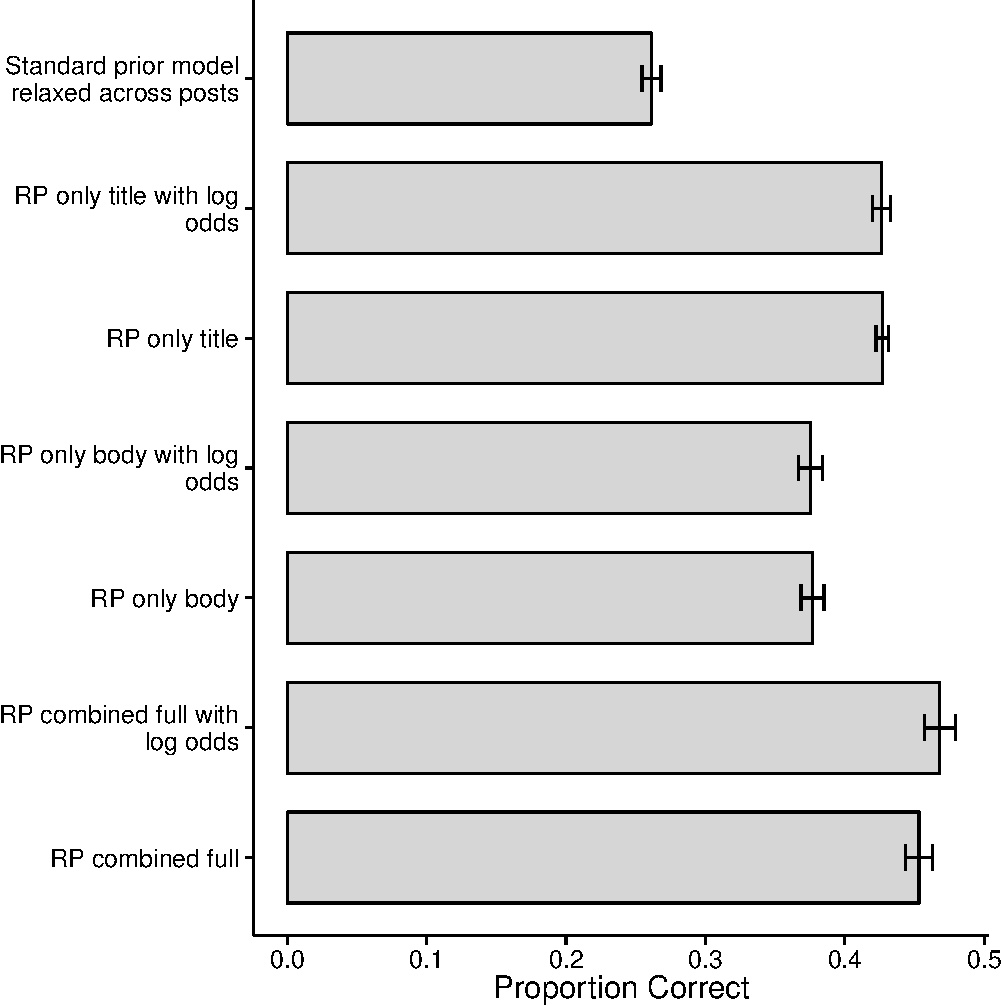
\includegraphics{compareMeanDV-acc-logoddsSO-crop.pdf}}}
  \caption{
    Random permutation model accuracy when using log-odds transformation on context for StackOverflow
    All error bars are the 95\% bootstrapped confidence interval for the mean. 
  }
  \label{figContextLogoddsSO}
\end{figure}

\begin{figure}[!htbp]
  \scalebox{.8}{\resizebox{\linewidth}{!}{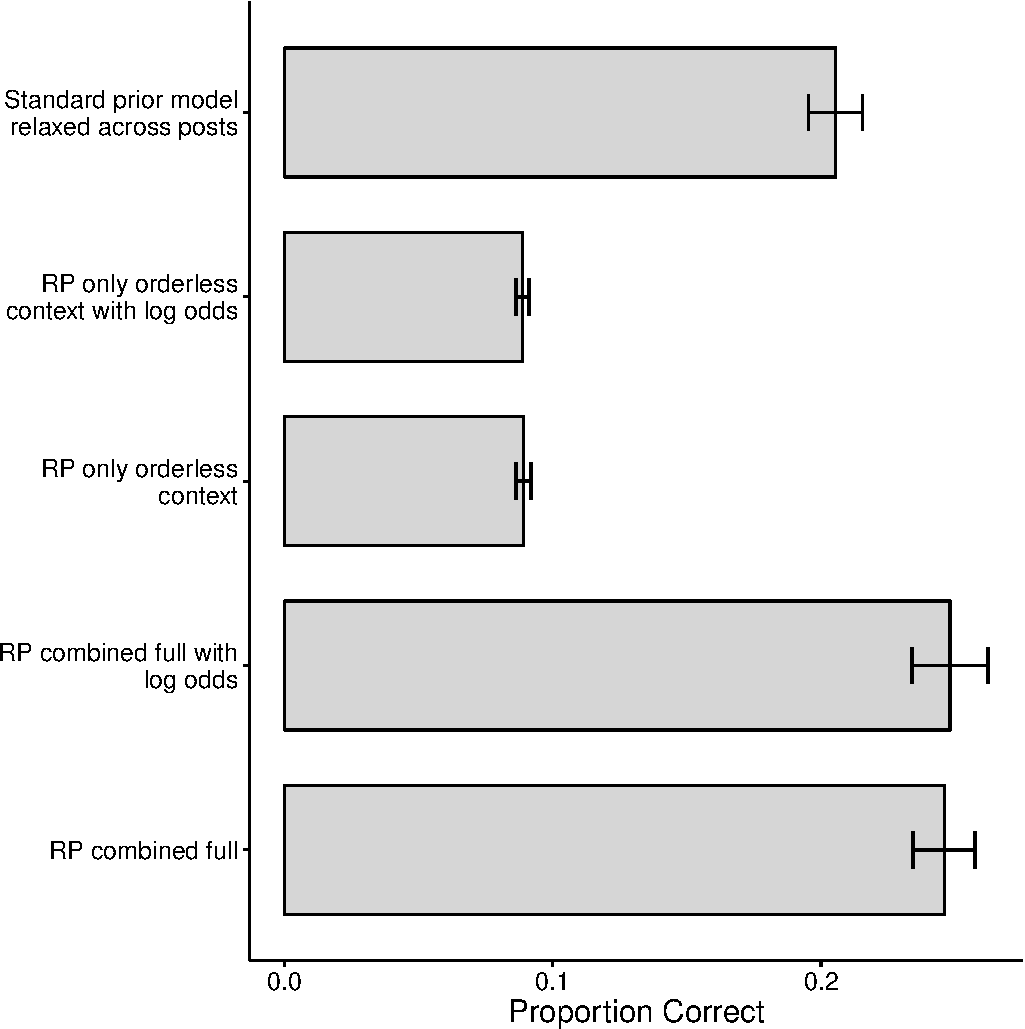
\includegraphics{compareMeanDV-acc-logoddsT-crop.pdf}}}
  \caption{
  Random permutation model accuracy when using log-odds transformation on context for Twitter
  All error bars are the 95\% bootstrapped confidence interval for the mean. 
}
  \label{figContextLogoddsT}
\end{figure}

\subsubsection{Discussion}

Vector-based models such as the random permutation model \parencite{Sahlgren2008} have included only a context component in the past (i.e., no prior component).
When the prior component is included for the random permutation model, accuracy improves significantly (compare accuracy for full models to context models in Figures \ref{figContextLogoddsSO} and \ref{figContextLogoddsT}).
However, it is somewhat surprising that it does not matter much how the context and prior terms are added for the random permutation model.
Model performance is similar when the context component used for the model is based on a correlation compared to a log-odds value.

There is a slight edge in increased accuracy when a log-odds transformation is used for the StackOverflow dataset, although the magnitude of the improvement in accuracy is small (\numNoZero{.45} to \numNoZero{.47}).
Nonetheless, it does seem appropriate to convert the context to a log-odds adjustment value when context is added as an additional term to the random permutation model.
Since performance does not decrease when the transformation is made, may slightly increase,
and leads to a more natural interpretation of each model term as a log-odds value, it is reasonable to include this step for the random permutation model.
Future research could explore additional methods to properly combine the terms.

\subsection{Word Order}

As a final architectural concern, vector-based models with and without word order were tested to examine the effect of word order on model accuracy.
Vector-based models like the random permutation model can easily incorporate word order when making predictions.
This has been touted as one of their primary strengths \parencites{Jones2007, Sahlgren2008}.
In order to thoroughly test the impact of adding word order into the model, various methods for incorporating word order were tested on the StackOverflow and Twitter datasets.

\subsubsection{Method}

Three different methods for incorporating word order in the random permutation model were tested:
taking just the sign of the word's position relative to the tag (direction method), using the position (standard method), and using the position but only including words that were used near the tag (window method).
For the standard method, all words and their respective position are used to build the representation.
For the direction method, essentially two representations are created: all co-occurrences with words to the left of the tag, and all co-occurrences with words to the right of the tag.
The window method is similar to the standard method, where each word's relative position is maintained, but it only includes words near the tag to build the representation.
\textcite{Sahlgren2008} tested similar methods, and found that accuracy was highest when a narrow window was used for the window method (only including words at most two positions to the left and right of the tag).
The same $+2$ $-2$ range was used to test the window method on the Twitter dataset.

Only the Twitter dataset was tested, since the StackOverflow dataset contains no word order information between words in the title and body of the post and the tags used for the post.
The author chooses tags after filling out the title and body forms in the post, so the tags are never intermixed with words in the post like they are for Twitter.

The same four Twitter popular-hashtags datasets were used for testing.
Both an ordered and orderless context component were created for the random permutation models.
The orderless context component uses the same co-occurrence matrix used by the Bayesian model to create the representation, since the Bayesian model does not contain any order information.
Models were tested that used only one of the three word order methods for the ordered context component, used only the orderless context component, used a combination of the two components, and combined context with prior. 

\subsubsection{Results}

Model accuracy results after incorporating word order into the random permutation model are depicted in Figure \ref{figContextOrder}.
All bar plots that include an order component where ``window'' or ``direction'' is not included in the title use the standard ordering method (no direction or windowing, all position information is included).
This is the default ordering method used, so the names for these bar plots were kept consistent to the names used in other figures so that comparisons could be made across figures.
Base models that do not use entropy weighting were also included so that effect sizes could be compared between entropy weighting and adding word order information.

\begin{figure}[!htbp]
  \scalebox{.8}{\resizebox{\linewidth}{!}{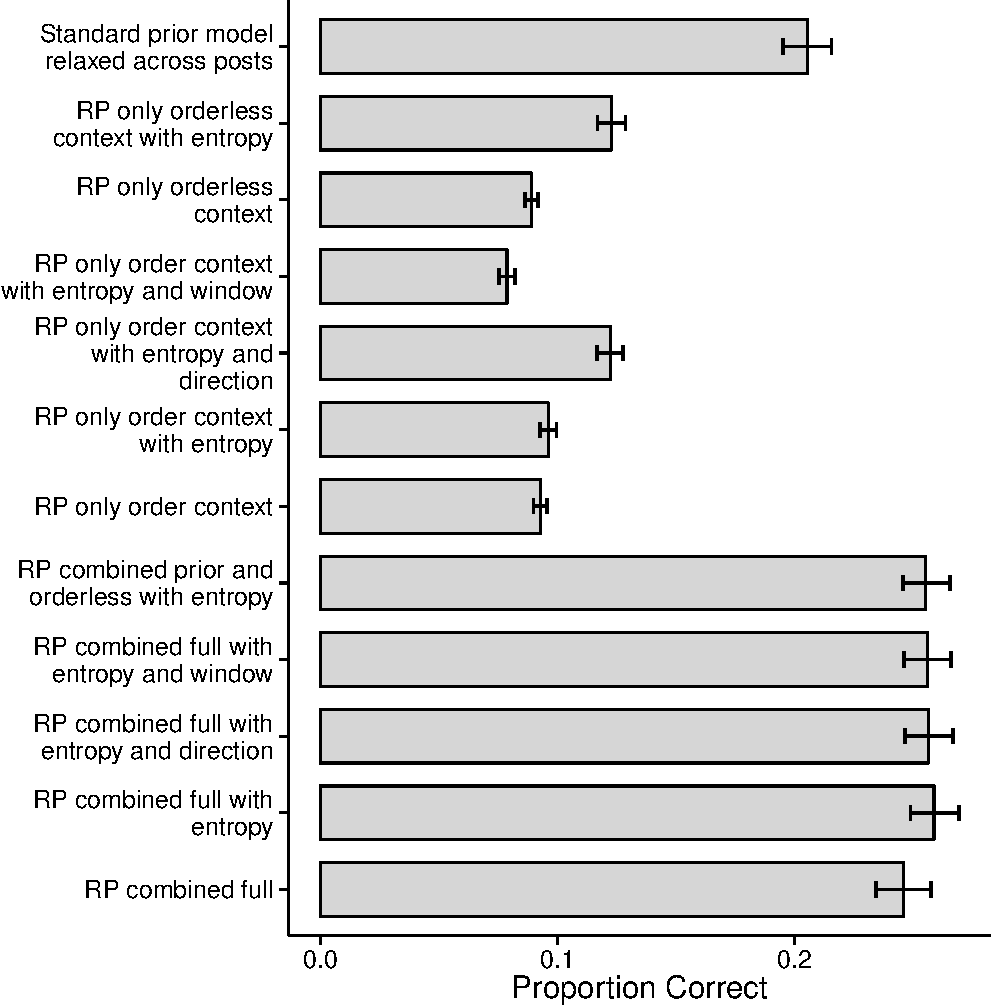
\includegraphics{compareMeanDV-acc-orderT-crop.pdf}}}
  \caption{
    Model accuracy for various word order methods for the random permutation model for Twitter
    All error bars are the 95\% bootstrapped confidence interval for the mean. 
  }
  \label{figContextOrder}
\end{figure}

Looking first at models where no prior is added, the random permutation model using only orderless context performs similar to the model using only order context with direction.
All other order-only models perform worse than the order model using direction and worse than the orderless model.

Full models were also plotted against the model where only the prior and orderless context was included (i.e., no order).
This was to test how much of the variance in model accuracy is shared between the orderless and order models.
The results show that there is little unique variance in the order-only models, so order information contributes little to overall model performance above and beyond what an orderless model contributes.
This can be seen by comparing the two-component model with only prior and orderless context to the three-component model with prior, orderless, and any of the three methods for the order context term.

\subsubsection{Discussion}

This was a surprising result.
One of the main benefits touted for the random permutation model is that it can easily incorporate word order information into the representation.
But including word order information does not dramatically improve performance. 
For the random permutation model, it is much more important to properly handle low-predictor stop words and include a prior component than it is to include word order information,
at least for the Twitter dataset tested in this study.

The original BEAGLE model \parencite{Jones2007} actually showed only minimal improvement when incorporating word order as well.
In absolute terms, this model only improved by 2 percentage points in accuracy when trained on the TASA and tested on the TOEFL.
\textcite{Sahlgren2008}'s results for word order for the random permutation model are similar.
At a row size of around \num{2000}, model accuracy improves by less than a percentage point when order information is incorporated.

Although incorporating word order into the random permutation model does seem to slightly improve performance,
the strength of the model is more likely to be in how efficiently it can represent the co-occurrence matrix rather than its ability to include word order in the representation.
That is, the strength of the model is in its compressed unordered context component term and not the ordered component, at least for the Twitter dataset studied.

Also, the reason why the directional version of ordering is the best predictor of the three ordered components is most likely because order information does not have a large effect,
so the two representations for words to the left and right of a tag are highly correlated.
This means that this directionally-ordered component is essentially composed of all the co-occurrence observations in the orderless component after being randomly sampled and partitioned into two separate representations.
The co-occurrences in these representations are highly correlated with each other, and highly correlated with the orderless component,
which is why model accuracy is similar for the orderless component and direction ordered component, and why accuracy does not improve when adding the direction ordered component to the orderless component.

\section{General Discussion}

The general discussion is separated into two parts.
The first section will describe the overall results,
and the final section will go through each key finding and discuss theoretical implications and future directions for research.

\subsection{Overall Results}

Table \ref{tabOverallResults} summarizes model accuracies for all models and datasets tested in the study.
This includes the prior-only model tested on the popular-users dataset and the full models (context and prior) tested on the popular-hashtags and randomly-sampled datasets.
After modifying the models by adding an entropy weighting mechanism to both models and a prior term to the random permutation model,
accuracy for the compressed random permutation model was nearly equal to the Bayesian model.
The largest difference between the two models was on the Twitter popular-hashtags dataset (7 percent).
Both models performed nearly equal for the StackOverflow datasets tested,
and both models were much more accurate when tested on StackOverflow compared to Twitter.

\begin{table}[!ht]
  \caption{
    Summary of accuracy for each model and dataset.
    The Bayesian model includes entropy weighting for the context words,
    the RP model includes entropy weighting and log odds transformation when combining the context and prior components.
  }
  \label{tabOverallResults}
  {\tabulinesep=1.2mm
    \begin{tabu}{llll}
      \hline
	Site 		& Dataset		& Model						& Accuracy \\
	\hline
	StackOverflow	& popular-users		& Standard prior model				& \numNoZero{.28} \\
			& randomly-sampled	& Bayesian with entropy 			& \numNoZero{.63} \\
			& 			& RP with entropy and log odds			& \numNoZero{.63} \\
	Twitter		& popular-users		& Standard prior model				& \numNoZero{.37} \\
			& popular-hashtags	& Bayesian with entropy				& \numNoZero{.32} \\
			& 			& RP with entropy and log odds			& \numNoZero{.25} \\
	\hline
    \end{tabu}
  }
\end{table}

\subsection{Implications and Future Directions}

\subsubsection{Tagging as a Declarative Memory Retrieval Process}

Overall, both the random permutation and Bayesian declarative memory models fit the observed tagging behavior in StackOverflow and Twitter reasonably well.
The fits for StackOverflow in particular are quite high, especially given the large tag space on the site.

These results provide support for the idea that choosing a hashtag when composing a tweet and tagging a StackOverflow post is akin to a declarative memory retrieval process.
However, both models are not 100 percent accurate, and the amount of variance left to predict is larger than what would be observed if retrieval noise is included in the model.
One possibility that seems likely is that the tag selection process includes other processes besides just declarative memory retrieval
(e.g., strategic processes, determining the number of tags to employ, attempts to add humor).

Another possibility is that this is not a declarative memory process at all.
In particular, it is important to note that tagging on these sites is widely used as a method to communicate specific messages to specific groups of people in the community.
It is unclear how much this environment overlaps with verbal communication between two people, and the declarative memory requests required to successfully communicate in this setting.
Nonetheless, these models are reasonably accurate in this setting, particularly for StackOverflow.
Given the results in this research, it at least seems worthwhile to use these publicly-available tagging environments as a reasonable proxy to explore and validate modifications to the current theory.

\subsubsection{Representation}

Given that the storage space required to represent the co-occurrences for the random permutation model is dramatically smaller than the uncompressed Bayesian model,
and that the compression is lossy and essentially random (i.e., no SVD),
it is quite interesting that the random permutation model performs nearly as well as the full Bayesian model for this task.

These results pose an interesting and important fundamental question about declarative memory:
How, precisely, is the neural system configured to represent co-occurrences for declarative memory?
Since at the behavioral level both models perform similarly, it is possible that the neural system is using something similar to either representation to store co-occurrences.
Vector-based models are simple enough that they can easily be implemented in a neural network.
Perhaps a form of vector-based compressed storage is being used at the neural level,
since it can be implemented in neurons and is an efficient way for the machinery to generate predictions that closely match the statistical structure of the environment
(i.e., that closely match the uncompressed Bayesian representation).

\subsubsection{Compression}

As previously noted, compression for the random permutation model is essentially random.
That is, no SVD is done to identify the most predictive components,
so the compressed representation used by the random permutation model does not contain nearly as much of the variance from the original co-occurrence matrix than it could have.
However, performing a full SVD on a co-occurrence matrix as large as the ones generated for StackOverflow and Twitter is computationally infeasible.
Also, when deriving the LSA approach, \textcite{Landauer1997} explicitly state that they make no claims that the brain is computing an SVD at the neural level;
only that the neural machinery is set up such that the representation makes predictions that are similar to what would have been generated if the matrix decomposition for an SVD would have been computed.
Perhaps the randomly-compressed representation used for the random permutation model is the way in which the brain tries to efficiently achieve the full LSA- and SVD-like approach that \citeauthor{Landauer1997} propose.

\subsubsection{Word Order}

The relatively strong performance of the random permutation model is not due to the model's ability to represent word order.
Performance is similar for the random permutation and Bayesian models when the co-occurrence matrix for both models is the same, and not based on word order.
Performance also does not improve by much when word order is added as the last predictor in the random permutation model.
The random permutation model seems to work so well mainly due to the way that the full co-occurrence representation is compressed.

\subsubsection{Corpus Size}

The random permutation model was more accurate than the Bayesian model at smaller corpus sizes, while the results were flipped for larger document sizes.
This is interesting from a practical standpoint because the corpus size is rarely chosen in declarative memory research, and is constrained mainly by the amount of data available in the domain being studied.
If a researcher is working within a domain that has a relatively small corpus size (generally near or less than \num{1000} documents),
it may be worthwhile to test the random permutation model in this domain, as this compressed model may be more accurate than the uncompressed Bayesian model.

Further, it is interesting to study the effect of model accuracy on corpus size because people require exposure to only a small number of documents before tagging documents appropriately.
On StackOverflow, each user asked an average of five questions.
Model accuracy was high for StackOverflow, but the model required training on 1 million documents before achieving that accuracy.
The user only needed to ``train'' on five questions and the model needed to train on 1 million questions.

This is a large discrepancy, but this does not necessarily invalidate the declarative memory models used for this research.
First, the random permutation model was still accurate at smaller document sizes, so perhaps this result provides evidence to favor the random permutation model over the Bayesian model.
However, the smallest corpus size tested for these models was \num{1000} documents, which is much greater than the average number of questions or tweets that a user contributes to the site.

Second, the models may require large amounts of training because the co-occurrence matrices are being built from scratch.
That is, the models are being trained on the StackOverflow and Twitter domains without any prior general co-occurrence information to start with.
Presumably, when a person starts using a site, they can leverage all of their past exposure to different word co-occurrences and then simply add on top of that base the domain-specific co-occurrences.
In that sense, one could argue that the models are undertrained on generic co-occurrences (people are exposed to many more than one million documents in their lifetime) and overtrained on specific co-occurrences.
It may be interesting to test these memory models on a hybrid co-occurrence matrix,
where the majority of the observations are taken from a generic domain (e.g., american literature) and a minority are domain-specific (e.g., StackOverflow word, tag pairs).

\subsubsection{Individual vs. Group Representation of Memory}

Even with the large datasets used in this research, there was not enough data on each individual user to build up separate co-occurrence matrices for them.
That is, the context component of the declarative memory models used in this research was formed as a collection of observed co-occurrences across all individuals.
Nonetheless, the prior component for the models was customized for each individual (except in the Twitter popular hashtags dataset when it was not possible).
Ideally, both components would be customized to the individual, and it remains an open question how much accuracy is influenced by using an aggregate or custom context component in the models.

\subsubsection{Attentional Weight}

The Bayesian declarative memory model for ACT-R has an attentional weight term $W_{j}$ that can be used to attenuate or remove stop words.
The random permutation model was also easily modified to have an attentional weight term by attenuating each word's set of ones and negative ones values by that word's attentional weight.
Both a method for stop-word removal (frequency filtering) and stop-word attenuating (entropy weighting) performed well for both models.

It is unclear at this point if this modification is cognitively plausible, even if the modification was cleanly added to the current ACT-R model.
What can be said from this research is that using a proper method for handling the low-predictor words produced some of the largest improvements in model accuracy compared to the other explorations
(e.g., compared to word order or properly adding terms).
Consequently, it may be worthwhile to explore this area more thoroughly in the future.

Also, there may be other ways besides adjusting the attentional weight that these models can be modified to achieve the same performance improvement.
The entropy weighting term is likely solving a problem that resides only in contextual activation and not prior activation,
since the activation for the prior component for each word is independent of the presentation of other words, so stop words have no way to interact with tag prior activation in this case.

One alternative explanation is that the entropy weighting measure was needed because the contextual co-occurrence matrix was not yet stable, even with these large dataset sizes.
If the matrix was not yet stable, then by chance certain stop words would contribute more net activation to specific tags and introduce noise into the retrieval process for that tag.
So further weighting the contribution of these stop words by leveraging the attentional weight term ensured that this noise was suppressed in the system.
If this is the case, it would be interesting to see how large a dataset is required to not need to modify the attentional weight term.
However even if this is the case, the random permutation model would still require entropy weighting for larger dataset sizes,
since this model simply adds environment vectors to produce the current context vector and has no mechanism (unlike Bayesian normalization) for weighting the contribution of an environment vector.

Another explanation for the Bayesian model is that additional attentional weighting was needed because the contextual matrix was derived only from word by tag co-occurrences and not (word or tag) by (word or tag) co-occurrences.
This was done for performance reasons as the computational complexity otherwise is simply too high for current hardware.
It is possible that by adding all pairwise combinations of both words and tags in the posts may soften and stabilize the contribution of stop words when computing contextual activation for a tag, given current context.

Also perhaps a different $S_{ji}$ model may not need entropy weighing at all (e.g., the Hebbian-inspired associative learning model described in \noparencite{thomson2013constraining}).
Further research could explore how entropy weighting interacts with other models of $S_{ji}$, and not just the random permutation and full Bayesian model.

Nonetheless, it seems likely that the entropy method for computing the attentional weight term $W_{j}$ may be applicable to other declarative memory tasks.
The entropy method is parameter-free (unlike the frequency-filtering method), completely data driven (much like the co-occurrence matrix), does not require tuning,
and increases model accuracy for these datasets.
It is common to handle stop words in some manner when working with Natural Language Processing (NLP) and large text corpuses.
So, if these large corpuses are used to test declarative memory,
then the entropy method may be a more cognitively plausible way of dealing with stop words rather than filtering based on a predetermined list or the frequency count in the dataset.

\subsubsection{Prior Component}

Adding a prior component to the random permutation model also increased model accuracy for both StackOverflow and Twitter.
It is unsurprising that this occurred.
However, it is quite surprising that this is the first time that the prior component has been included and tested in a random permutation model.
If the random permutation model is explored as a declarative memory theory for other datasets, it should be worthwhile to include the prior component for those explorations.
Although it did not seem to matter much how the prior component is combined with the context component in this study, 
there may be better ways than the log-odds transformation to combine the terms.
Further research could focus on exploring a larger set of methods for combining the context component of the random permutation model with the prior component from the ACT-R theory.

\subsubsection{Activation Calculation}

The Bayesian and vector-based memory models differ in how the co-occurrence matrix is represented (lossy compression for vector-based models).
They also differ in how the activation of each tag is calculated, given the different representations.
The vector-based memory models, like LSA, compute a correlation between the context and each tag, while the Bayesian models sum the log likelihoods that each word in the context occurs with each tag.
These two methods for computing the activation are correlated but not identical.
Further research could try to tease apart how model accuracy is independently influenced by the representation (compressed or not) and the activation calculation (correlation or log likelihood).
To do this, four models could be constructed (uncompressed and compressed representation crossed with correlation and log likelihood activation) compared to the two in this study,
so that the effects of representation and activation calculation could be partialed out.
This would allow, for example, the method of compression for the random permutation vector-based model to be analyzed independent of activation calculation.
The results would help determine the specific representation that the declarative memory system uses to represent co-occurrences,
and also the specific activation calculation that is carried out by the system.

\subsubsection{Observational vs. Experimental Design}

All data used for this study were collected from publicly-available datasets and were not subject to an experimental design (i.e., observational data).
There are advantages and disadvantages to both observational and experimental designs.
One primary advantage with the observational approach here is size and availability: data for millions of posts and tweets are immediately available for analysis.
However one disadvantage is that there is no way to probe a user at a particular point in time, which could be quite advantageous for answering certain questions.
One hybrid approach worth considering for future research is to use the publicly available datasets to build up a representation of declarative memory for each user.
Afterwards, bring a sample of these specific users into a laboratory setting and probe them with specific retrieval requests.
Multiple users could be asked to tag the same message, and then models could be tested to see if they reliably predict differences in accuracy between the subjects.

\subsubsection{Directly Comparing the Models}

After including the prior and entropy components for both models, overall accuracy was similar for the Bayesian and random permutation models for this task.
So it is unclear precisely which model is more cognitively plausible (or if both are correct and simply working at different levels of abstraction).
However, there were two areas in particular where model performance showed relatively large differences: accuracy change as a function of corpus size and reliance on entropy weighting.
These areas could be used in future research to more directly challenge the models.
For example, a domain could be picked where enough data is collected to build a custom co-occurrence matrix for each user.
Then one could look at model accuracy over time for each user as the co-occurrence matrix is increased to see if the trajectory is more accurately modeled by a random permutation (more accurate with lower N) or Bayesian (more accurate with higher N) model.
Further, if a large-scale domain is picked and it is shown that the Bayesian model does not require entropy weighting for the co-occurrence matrix after the representations are fully stabilized,
then this would provide a case where the two models are dramatically different: The random permutation model would require explicitly weighting the stop words (entropy weighting) while the Bayesian model would not.

\subsection{Summary}

This work has shown how large collections of publicly-available behavioral data can be used to explore and test different theories of declarative memory and their individual architectural components.
This in turn provided [1] a better understanding of how a user's past tagging history influences future tag use,
[2] a more thorough evaluation of the strengths, weaknesses, and differences between two cognitively-plausible memory models on large-scale real-world retrieval tasks,
and [3] two efficient implementations of the models for making user-customized tag predictions for StackOverflow posts and Twitter tweets. 

This work has shown how past user history is important, and how a context-only model like the random permutation model can be modified to include the prior component.
The work has also shown how the strength of the random permutation model may not be in its ability to represent word order,
but rather in its ability to efficiently compress the full co-occurrence representation used for the Bayesian model.
Several different formalisms for ACT-R's attentional weighting term were also explored, and an entropy-weighting technique was found to perform well without requiring any parameter tuning.
Finally, this work has helped raise the question about how co-occurrence observations are represented at the neural level, since two models with quite different representations performed similarly well.
The results from the study and the new research questions raised will help to better understand how imposing specific architectural constraints on memory models influence what information is retrieved.

\clearpage
\printbibliography[heading=bibintoc]

\end{document}

